\documentclass{openETCS/openetcs}
% Use the option "nocc" if the document is not licensed under Creative Commons
%\documentclass[nocc]{template/openetcs}
\usepackage{lipsum,url}
\usepackage{supertabular}
\usepackage{multirow}
\usepackage{color, colortbl}
\usepackage{listings}
\definecolor{gray}{rgb}{0.8,0.8,0.8}
\usepackage[modulo]{lineno}
\graphicspath{{./openETCS/}{.}{./image/}}
\begin{document}
\frontmatter
\project{openETCS}

%Please do not change anything above this line
%============================

% The document metadata is defined below

%assign a report number here
\reportnum{OETCS/WP5/M5.3}

%define your workpackage here
\wp{Work-Package 5: ``Demonstrator''}

%set a title here
\title{Automatic Test Runner User manual}

%set a subtitle here
\subtitle{A comprehensive guide for writing and running SRS 330 scenarios.}

%set the date of the report here
\date{February 2015}


%document approval
%define the name and affiliation of the people involved in the documents approbation here
\creatorname{Didier Weckmann}
\creatoraffil{ERSA}

\techassessorname{Didier Weckmann}
\techassessoraffil{ERSA}

\qualityassessorname{Ainhoa Gracia}
\qualityassessoraffil{SQS}

\approvalname{Klaus-R\"udiger Hase}
\approvalaffil{DB Netz}


%define a list of authors and their affiliation here

\author{Alexis Julin, Didier Weckmann, Nicolas Van Landeghem}

\affiliation{ERSA\\
  5 Rue Maurice Blin \\
  67500 Haguenau, France}

% define the coverart
\coverart[width=350pt]{openETCS_EUPL}

%define the type of report
\reporttype{Description of work}

\begin{abstract}
	%define an abstract here
	This document present how the Automatic Test Runner can be used to execute Baseline 3 scenarios. This document also describe the scenario file format and its syntax.
\end{abstract}

%=============================
\maketitle

%Modification history
%if you do not need a modification history table for your document simply comment out the eight lines below
%=============================


\section*{Modification History}
\tablefirsthead{
	\hline 
	\rowcolor{gray} 
	Version & Section & Modification / Description & Author \\\hline}
\begin{supertabular}{| m{1.2cm} | m{1.2cm} | m{6.6cm} | m{4cm} |}
	0.1 &All parts&Creation &Christophe Menager \\\hline
	1.0 &All parts&Official version &Christophe Menager \\\hline
	1.1 &All parts&Add option to set SRS language for message &Eric Schellenberg \\\hline
	2.0 &All parts&Update for new version with integrated DMI &Christophe Menager \\\hline
	2.1 &All parts&Correction of driver action &Eric Schellenberg \\\hline
	2.2 &All parts&Added new WAIT\_ICON and BUTTON commands &Flavien Bridault \\\hline
	2.3 &All parts&REGENBRK\_ON/OFF,  EDDYCURRBRK\_ON/OFF, MAGNSHOEBRK\_ON/OFF descriptions were erroneous and didn’t reflect reality in code &Didier Weckmann \\\hline
	2.4 &All parts&NTC\_MODULE in Config\_EVCInit &Flavien Bridault \\\hline
	2.5 &All parts&Config\_Scenario section &Flavien Bridault \\\hline
	2.6 &All parts&Add tests for speed monitoring status &Stéphane Chenevoy \\\hline
	2.7 &All parts&Add WAIT\_DYNAMIC commands &Didier Weckmann \\\hline
	2.8 &All parts&Add EXPECTED\_TO\_FAIL command &Didier Weckmann \\\hline
	2.9 &All parts&Add WAIT\_BUTTON ACK\_XXX &Didier Weckmann \\\hline
	2.10 &All parts&Add EVC\_CONFIG, NV\_FROM\_HEX\_BUFFER and COUNTRIES\_ID &Alexis Julin \\\hline
	2.11 &All parts&Reply to GE comments &Didier Weckmann \\\hline
	2.12 &All parts&Add WAIT\_TEXT description&Alexis Julin \\\hline
	2.13 &All parts& Add CHECK\_TRACKCONDITION description&Alexis Julin \\\hline
\end{supertabular}


\tableofcontents
\listoffiguresandtables
\newpage
%=============================

%Uncomment the next line if you need line numbers for tracebility when the document is in review
%\linenumbers
%=============================


% The actual document starts below this line
%=============================

%Start here

%document content
\documentclass{template/openetcs}
% Use the option "nocc" if the document is not licensed under Creative Commons
%\documentclass[nocc]{template/openetcs}
\usepackage{lipsum,url}
\usepackage{supertabular}
\usepackage{multirow}
\usepackage{color, colortbl}
\usepackage{listings}
\definecolor{gray}{rgb}{0.8,0.8,0.8}
\usepackage[modulo]{lineno}
\graphicspath{{./template/}{.}{./images/}}
\begin{document}
\frontmatter
\project{openETCS}

%Please do not change anything above this line
%============================

% The document metadata is defined below

%assign a report number here
\reportnum{OETCS/WP5/M5.1}

%define your workpackage here
\wp{Work-Package 5: ``Demonstrator''}

%set a title here
\title{Automatic Test Runner User manual}

%set a subtitle here
\subtitle{A comprehensive guide for writing and running SRS 330 scenarios.}

%set the date of the report here
\date{June 2014}


%document approval
%define the name and affiliation of the people involved in the documents approbation here
\creatorname{Didier Weckmann}
\creatoraffil{ERSA}

\techassessorname{Didier Weckmann}
\techassessoraffil{ERSA}

\qualityassessorname{Ainhoa Gracia}
\qualityassessoraffil{SQS}

\approvalname{Klaus-R\"udiger Hase}
\approvalaffil{DB Netz}


%define a list of authors and their affiliation here

\author{Alexis Julin, Didier Weckmann, Nicolas Van Landeghem}

\affiliation{ERSA\\
  5 Rue Maurice Blin \\
  67500 Haguenau, France}

% define the coverart
\coverart[width=350pt]{openETCS_EUPL}

%define the type of report
\reporttype{Description of work}


\begin{abstract}
%define an abstract here
  This document present how the Automatic Test Runner can be used to execute Baseline 3 scenarios. This document also describe the scenario file format and its syntax.
\end{abstract}

%=============================
\maketitle

%Modification history
%if you do not need a modification history table for your document simply comment out the eight lines below
%=============================


\section*{Modification History}
\tablefirsthead{
\hline 
\rowcolor{gray} 
Version & Section & Modification / Description & Author \\\hline}
\begin{supertabular}{| m{1.2cm} | m{1.2cm} | m{6.6cm} | m{4cm} |}
0.1 &All parts&Creation &Christophe Menager \\\hline
1.0 &All parts&Official version &Christophe Menager \\\hline
1.1 &All parts&Add option to set SRS language for message &Eric Schellenberg \\\hline
2.0 &All parts&Update for new version with integrated DMI &Christophe Menager \\\hline
2.1 &All parts&Correction of driver action &Eric Schellenberg \\\hline
2.2 &All parts&Added new WAIT\_ICON and BUTTON commands &Flavien Bridault \\\hline
2.3 &All parts&REGENBRK\_ON/OFF,  EDDYCURRBRK\_ON/OFF, MAGNSHOEBRK\_ON/OFF descriptions were erroneous and didn’t reflect reality in code &Didier Weckmann \\\hline
2.4 &All parts&NTC\_MODULE in Config\_EVCInit &Flavien Bridault \\\hline
2.5 &All parts&Config\_Scenario section &Flavien Bridault \\\hline
2.6 &All parts&Add tests for speed monitoring status &Stéphane Chenevoy \\\hline
2.7 &All parts&Add WAIT\_DYNAMIC commands &Didier Weckmann \\\hline
2.8 &All parts&Add EXPECTED\_TO\_FAIL command &Didier Weckmann \\\hline
2.9 &All parts&Add WAIT\_BUTTON ACK\_XXX &Didier Weckmann \\\hline
2.10 &All parts&Add EVC\_CONFIG, NV\_FROM\_HEX\_BUFFER and COUNTRIES\_ID &Alexis Julin \\\hline
2.11 &All parts&Reply to GE comments &Didier Weckmann \\\hline
\end{supertabular}


\tableofcontents
\listoffiguresandtables
\newpage
%=============================

%Uncomment the next line if you need line numbers for tracebility when the document is in review
%\linenumbers
%=============================


% The actual document starts below this line
%=============================

%Start here

\section{Introduction}

This document explains how to use the Automatic Test Runner.

The purpose of the Automatic Test Runner is to provide a tool that allows the automatic tests of the on-board simulator with a set of scenarios during developments in order to validate the changes and perform non regression tests.

The tester is a graphical application integrating an on-board and a simplified DMI. It can simulate all interfaces to the EVC (e.g. balises, radio, loops, odometer, TIU and driver interfaces). It can test the internal state of on-board in order to check its correct behaviour according to an input scenario.

In a first step, this document only concerns the simulated demonstrator. Indeed, the physical demonstrator will be available in a second step. Thus, the document will be updated accordingly.

\section{How to create scenarios}
\subsection{Introduction}

A scenario is a text file containing the description of interactions with the on-board and test conditions on the on-board internal states and/or outputs (TIU, radio message)
The scenario describes how the Automatic Test Runner has to stimulate the interfaces of the on-board:

\begin{itemize}
	\item Odometer: by simulating a train movement according to a given speed profile.
	\item Train interface: by simulating the train device inputs to the on-board.
	\item Driver: by simulating actions of the driver on a driver machine interface (DMI).
	\item Balise: by simulating the emission of balise contents to the on-board.
	\item Loop: by simulating the emission of loop contents to the on-board.
	\item Radio: by simulating radio communication from RBC/RIU to on-board.
\end{itemize}

According to the described interactions, a defined behaviour of the on-board is awaited and test conditions can be described in the scenario in order to test the internal state of the on-board and validate the awaited behaviour. These test conditions are defined later in the document and have different trigger: waiting a preset time, waiting a preset location, waiting a predefined output, ... 

Note: The file extension for scenario files is ‘.sce’.
\newline
Note 2: The STM module is out of the openETCS project scope and will not be handled within this document.

\subsection{Scenario file description}

A scenario file is composed of several sections which are indicated in the file between brackets: “[<section name>]”.

Here is the list of the different section names:

\begin{description}
	\item[SCENARIO:] Main section for the scenario execution.
	\item[SpeedProfile:] Description of the speed profile used for train movement simulation.
	\item[BaliseTrackside:] Description of balise contents to be sent to on-board.
	\item[LoopTrackside:] Description of loop messages to be sent to on-board.
	\item[Config\_SRSNationalDefaults:] Description of the default national values used by on-board.
	\item[Config\_EVCInit:] Description of starting conditions used by on-board.
	\item[Config\_TrainData:] Description of train data used by on-board. 
	\item[Config\_RBCData1:] Description of the first RBC parameters used for testing. 
	\item[Config\_RBCData2:] Description of the second RBC parameters used for testing. 
	\item[Config\_Scenario:] Specific options for the testrunner about the current scenario.
\end{description}

FixedData refer to SRS section A3.1. To improve the EVC testability, it is also possible to specify other values, e.g. SAFECONNECTION\_TIMEOUT or MAX\_RECONNECTION\_TIME can be shorten.

For data defined within SRS packets, these have to be set using the dedicated SRS message (e.g. gradient profile is defined within packet 21).

The user can also define its own sections for balise, loop and radio message contents and radio execution thread.

Comments lines can be added in the scenario file using “\#”.
If some data of section Config\_SRSNationalDefaults, Config\_FixedData, Config\_EVCInit or Config\_TrainData are not defined, default values are used (see the corresponding chapter for more information about the default values).

\subsubsection{Scenario inclusion}

It is possible to include files in a scenario file when common sections are used. This can be done anywhere in the file by using the ‘INCLUDE’ keyword as follows: 

\emph{\texttt{INCLUDE=<file>}}

\subsubsection{Main section: SCENARIO}

This section is composed of a succession of commands. These commands can request different type of actions:

\begin{itemize}
	\item DRIVER\_ACTION:
	
		\begin{longtable}{|l|l|l|}
			\caption{DRIVER\_ACTION}\\  
			\hline
	
				\begin{minipage}[t]{0.22\linewidth} \textbf{Description} \end{minipage} 
			&	\multicolumn{2}{l|}{ \begin{minipage}[t]{0.78\linewidth} Simulates a driver actions interacting with the EVC (DMI or TIU interfaces). Optionally the scenario execution can be suspended a given time delay before executing next command. \end{minipage} } \\
			
			\hline
						
				\begin{minipage}[t]{0.22\linewidth} \textbf{Syntax}	\end{minipage}
			&	\multicolumn{2}{l|}{ \begin{minipage}[t]{0.78\linewidth} \emph{\texttt{DRIVER\_ACTION = <Action>, <Delay>}}	\end{minipage} } \\
			
			\hline
		
				\multirow{1}{*}{ \begin{minipage}[t]{0.22\linewidth} \textbf{<Action>} \end{minipage} }
			&	\multicolumn{2}{l|}{ \begin{minipage}[t]{0.78\linewidth} <Action> on the DMI: \end{minipage} } \\
			
			\hline
			
			&	\begin{minipage}[t]{0.40\linewidth} \emph{\texttt{Level0}} \end{minipage}
			&	\begin{minipage}[t]{0.38\linewidth} ETCS level 0 entry \end{minipage} \\
			
			\hline
			
			&	\begin{minipage}[t]{0.40\linewidth} \emph{\texttt{Level1}} \end{minipage}
			&	\begin{minipage}[t]{0.38\linewidth} ETCS level 1 entry \end{minipage} \\
			
			\hline
			
			&	\begin{minipage}[t]{0.40\linewidth} \emph{\texttt{Level2}} \end{minipage}
			&	\begin{minipage}[t]{0.38\linewidth} ETCS level 2 entry \end{minipage} \\
			
			\hline
			
			&	\begin{minipage}[t]{0.40\linewidth} \emph{\texttt{Level3}} \end{minipage}
			&	\begin{minipage}[t]{0.38\linewidth} ETCS level 3 entry \end{minipage} \\ 
			
			\hline
			
			&	\begin{minipage}[t]{0.40\linewidth} \emph{\texttt{DriverID}} \end{minipage}
			&	\begin{minipage}[t]{0.38\linewidth} Driver identifier entry \end{minipage} \\
			
			\hline
			
			&	\begin{minipage}[t]{0.40\linewidth} \emph{\texttt{TrainRunningNumber}} \end{minipage}
			&	\begin{minipage}[t]{0.38\linewidth} Train running number entry \end{minipage} \\
			
			\hline
			
			&	\begin{minipage}[t]{0.40\linewidth} \emph{\texttt{TrainData}} \end{minipage}
			&	\begin{minipage}[t]{0.38\linewidth} Train data entry \end{minipage} \\
			
			\hline
			
			&	\begin{minipage}[t]{0.40\linewidth} \emph{\texttt{TrainData+TRN}} \end{minipage}
			&	\begin{minipage}[t]{0.38\linewidth} Train data entry with train running number entry \end{minipage} \\
			
			\hline
			
			&	\begin{minipage}[t]{0.40\linewidth} \emph{\texttt{StartOfMission}} \end{minipage}
			&	\begin{minipage}[t]{0.38\linewidth} Start of mission request \end{minipage} \\
			
			\hline
			
			&	\begin{minipage}[t]{0.40\linewidth} \emph{\texttt{NonLeadingModeEntry}} \end{minipage}
			&	\begin{minipage}[t]{0.38\linewidth} Non leading entry request \end{minipage} \\
			
			\hline
			
			&	\begin{minipage}[t]{0.40\linewidth} \emph{\texttt{NonLeadingModeExit}} \end{minipage}
			&	\begin{minipage}[t]{0.38\linewidth} Non leading exit request \end{minipage} \\
			
			\hline
			
			&	\begin{minipage}[t]{0.40\linewidth} \emph{\texttt{ShuntingModeEntry}} \end{minipage}
			&	\begin{minipage}[t]{0.38\linewidth} Shunting entry request \end{minipage} \\
			
			\hline
			
			&	\begin{minipage}[t]{0.40\linewidth} \emph{\texttt{ShuntingModeExit}} \end{minipage}
			&	\begin{minipage}[t]{0.38\linewidth}Shunting exit request \end{minipage} \\
			
			\hline
			
			&	\begin{minipage}[t]{0.40\linewidth} \emph{\texttt{OverrideEOA}} \end{minipage}
			&	\begin{minipage}[t]{0.38\linewidth} Request to override EOA \end{minipage} \\
			
			\hline
			
			&	\begin{minipage}[t]{0.40\linewidth} \emph{\texttt{OverrideUnsuitability}} \end{minipage}
			&	\begin{minipage}[t]{0.38\linewidth} Request to override route unsuitability \end{minipage} \\
			
			\hline
			
			&	\begin{minipage}[t]{0.40\linewidth} \emph{\texttt{AckBrake}} \end{minipage}
			&	\begin{minipage}[t]{0.38\linewidth} Acknowledgement for brake icon \end{minipage} \\
			
			\hline
			
			&	\begin{minipage}[t]{0.40\linewidth} \emph{\texttt{AckMessage}} \end{minipage}
			&	\begin{minipage}[t]{0.38\linewidth} Acknowledgement for message \end{minipage} \\
			
			\hline
			
			&	\begin{minipage}[t]{0.40\linewidth} \emph{\texttt{AckModeOrLevel}} \end{minipage}
			&	\begin{minipage}[t]{0.38\linewidth} Acknowledgement for mode/Level icon \end{minipage} \\
			
			\hline
			
			&	\begin{minipage}[t]{0.40\linewidth} \emph{\texttt{AckTAF}} \end{minipage}
			&	\begin{minipage}[t]{0.38\linewidth} Acknowledgement for track ahead free \end{minipage} \\
			
			\hline
			
			&	\begin{minipage}[t]{0.40\linewidth} \emph{\texttt{ConfirmIntegrity}} \end{minipage}
			&	\begin{minipage}[t]{0.38\linewidth} Confirm integrity \end{minipage} \\
			
			\hline
			
			&	\begin{minipage}[t]{0.40\linewidth} \emph{\texttt{EnterLevel}} \end{minipage}
			&	\begin{minipage}[t]{0.38\linewidth} Open level menu \end{minipage} \\
			
			\hline
			
			&	\begin{minipage}[t]{0.40\linewidth} \emph{\texttt{MainWindow}} \end{minipage}
			&	\begin{minipage}[t]{0.38\linewidth} Return to main window \end{minipage} \\
			
			\hline
			
			&	\begin{minipage}[t]{0.40\linewidth} \emph{\texttt{SlipperyTrack}} \end{minipage}
			&	\begin{minipage}[t]{0.38\linewidth} Select slippery track \end{minipage} \\
			
			\hline
			
			&	\begin{minipage}[t]{0.40\linewidth} \emph{\texttt{NonSlipperyTrack}} \end{minipage}
			&	\begin{minipage}[t]{0.38\linewidth} Select non slippery track \end{minipage} \\
			
			\hline
			
			&	\multicolumn{2}{l|}{ \begin{minipage}[t]{0.78\linewidth} <Action> on the TIU: \end{minipage} } \\
			
			\hline
			
			&	\begin{minipage}[t]{0.40\linewidth} \emph{\texttt{MainSwitchOn}} \end{minipage}
			&	\begin{minipage}[t]{0.38\linewidth} Set EVC power TIU input to ‘on’ \end{minipage} \\
			
			\hline
			
			&	\begin{minipage}[t]{0.40\linewidth} \emph{\texttt{MainSwitchOff}} \end{minipage}
			&	\begin{minipage}[t]{0.38\linewidth} Set EVC power TIU input to ‘off’\end{minipage} \\
			
			\hline
			
			&	\begin{minipage}[t]{0.40\linewidth} \emph{\texttt{TrainIntegrityOK}} \end{minipage}
			&	\begin{minipage}[t]{0.38\linewidth} Set integrity device TIU input to ‘OK’ \end{minipage}\\
			
			\hline
			
			&	\begin{minipage}[t]{0.40\linewidth} \emph{\texttt{TrainIntegrityNOK}} \end{minipage}
			&	\begin{minipage}[t]{0.38\linewidth} Set integrity device TIU input to ‘NOK’ \end{minipage} \\
			
			\hline
			
			&	\begin{minipage}[t]{0.40\linewidth} \emph{\texttt{OpenCabinA}} \end{minipage}
			&	\begin{minipage}[t]{0.38\linewidth} Set cabin status TIU input to ‘cabin A opened’ \end{minipage} \\
			
			\hline
			
			&	\begin{minipage}[t]{0.40\linewidth} \emph{\texttt{OpenCabinB}} \end{minipage}
			&	\begin{minipage}[t]{0.38\linewidth} Set cabin status TIU input to ‘cabin B opened’ \end{minipage} \\
			
			\hline
			
			&	\begin{minipage}[t]{0.40\linewidth} \emph{\texttt{CloseCabin}} \end{minipage}
			&	\begin{minipage}[t]{0.38\linewidth} Set cabin status TIU input to ‘no cabin opened’ \end{minipage} \\
			
			\hline
			
			&	\begin{minipage}[t]{0.40\linewidth} \emph{\texttt{EVCIsolationOn}} \end{minipage}
			&	\begin{minipage}[t]{0.38\linewidth} Swith to Isolation mode \end{minipage} \\
			
			\hline
			
			&	\begin{minipage}[t]{0.40\linewidth} \emph{\texttt{EVCIsolationReset}} \end{minipage}
			&	\begin{minipage}[t]{0.38\linewidth}v Reset Isolation mode \end{minipage} \\
			
			\hline
			
			&	\begin{minipage}[t]{0.40\linewidth} \emph{\texttt{EVCSleepingOn}} \end{minipage}
			&	\begin{minipage}[t]{0.38\linewidth} Set Sleeping TIU input to ‘on’ \end{minipage} \\
			
			\hline
			
			&	\begin{minipage}[t]{0.40\linewidth} \emph{\texttt{EVCSleepingOff}} \end{minipage}
			&	\begin{minipage}[t]{0.38\linewidth} Set sleeping TIU input to ‘off’\end{minipage} \\
			
			\hline
			
			&	\begin{minipage}[t]{0.40\linewidth} \emph{\texttt{ColdMovementDetectOn}} \end{minipage}
			&	\begin{minipage}[t]{0.38\linewidth} Set cold movement detector input to ‘on’ \end{minipage} \\
			
			\hline
			
			&	\begin{minipage}[t]{0.40\linewidth} \emph{\texttt{ColdMovementDetectOff}} \end{minipage}
			&	\begin{minipage}[t]{0.38\linewidth} Set cold movement detector input to ‘off’ \end{minipage} \\
			
			\hline
			
			&	\begin{minipage}[t]{0.40\linewidth} \emph{\texttt{DirectionNominal}} \end{minipage}
			&	\begin{minipage}[t]{0.38\linewidth} Set direction controller TIU input to ’Nominal’ (forward) \end{minipage} \\
			
			\hline
			
			&	\begin{minipage}[t]{0.40\linewidth} \emph{\texttt{DirectionReverse}} \end{minipage}
			&	\begin{minipage}[t]{0.38\linewidth} Set direction controller TIU input to ’Reverse’ (backward) \end{minipage} \\
			
			\hline
			
			&	\begin{minipage}[t]{0.40\linewidth} \emph{\texttt{DirectionStandstill}} \end{minipage}
			&	\begin{minipage}[t]{0.38\linewidth} Set direction controller TIU input to ’Standstill’ (neutral) \end{minipage} \\
			
			\hline
			
			&	\begin{minipage}[t]{0.40\linewidth} \emph{\texttt{DirectionUndefined}} \end{minipage}
			&	\begin{minipage}[t]{0.38\linewidth} Set direction controller TIU input to ’Undefined’ \end{minipage} \\
			
			\hline
			
			&	\begin{minipage}[t]{0.40\linewidth} \emph{\texttt{SBOn}} \end{minipage}
			&	\begin{minipage}[t]{0.38\linewidth} Set service brake TIU input to ’on’ \end{minipage} \\
			
			\hline
			
			&	\begin{minipage}[t]{0.40\linewidth} \emph{\texttt{SBOff}} \end{minipage}
			&	\begin{minipage}[t]{0.38\linewidth} Set service brake TIU input to ’off’ \end{minipage} \\
			
			\hline
			
			&	\begin{minipage}[t]{0.40\linewidth} \emph{\texttt{EBOn}} \end{minipage}
			&	\begin{minipage}[t]{0.38\linewidth} Set emergency brake TIU input to ’on’ \end{minipage} \\
			
			\hline
			
			&	\begin{minipage}[t]{0.40\linewidth} \emph{\texttt{EBOff}} \end{minipage}
			&	\begin{minipage}[t]{0.38\linewidth} Set emergency brake TIU input to ’off’ \end{minipage} \\
			
			\hline
			
			&	\begin{minipage}[t]{0.40\linewidth} \emph{\texttt{SBOutOfOrder}} \end{minipage}
			&	\begin{minipage}[t]{0.38\linewidth} Set service brake out of order \end{minipage} \\
			
			\hline
			
			&	\begin{minipage}[t]{0.40\linewidth} \emph{\texttt{EBOutOfOrder}} \end{minipage}
			&	\begin{minipage}[t]{0.38\linewidth} Set emergency brake out of order \end{minipage} \\
			
			\hline
			
			&	\begin{minipage}[t]{0.40\linewidth} \emph{\texttt{MCBOpen}} \end{minipage}
			&	\begin{minipage}[t]{0.38\linewidth} Set main circuit breaker TIU input to ’open’ \end{minipage} \\
			
			\hline
			
			&	\begin{minipage}[t]{0.40\linewidth} \emph{\texttt{MCBClose}} \end{minipage}
			&	\begin{minipage}[t]{0.38\linewidth} Set main circuit breaker TIU input to ’close’ \end{minipage} \\
			
			\hline
			
			&	\begin{minipage}[t]{0.40\linewidth} \emph{\texttt{PantographDown}} \end{minipage}
			&	\begin{minipage}[t]{0.38\linewidth} Set pantograph TIU input to ’down’ \end{minipage} \\
			
			\hline
			
			&	\begin{minipage}[t]{0.40\linewidth} \emph{\texttt{PantographUp}} \end{minipage}
			&	\begin{minipage}[t]{0.38\linewidth} Set pantograph TIU input to ’up’ \end{minipage} \\
			
			\hline
			
			&	\begin{minipage}[t]{0.40\linewidth} \emph{\texttt{PassengerEBOff}} \end{minipage}
			&	\begin{minipage}[t]{0.38\linewidth} Set passenger emergency brake TIU input to ’off’ \end{minipage} \\
			
			\hline
			
			&	\begin{minipage}[t]{0.40\linewidth} \emph{\texttt{PassengerEBOn}} \end{minipage}
			&	\begin{minipage}[t]{0.38\linewidth} Set passenger emergency brake TIU input to ’on’ \end{minipage} \\
			
			\hline
			
				\begin{minipage}[t]{0.22\linewidth} \textbf{<Delay>} \end{minipage}
			&	\multicolumn{2}{l|}{ \begin{minipage}[t]{0.78\linewidth} Time delay in seconds to wait before executing next command (optional) \end{minipage} } \\
			
			\hline
			
				\begin{minipage}[t]{0.22\linewidth} \textbf{Example} \end{minipage}
			&	\multicolumn{2}{l|}{ \begin{minipage}[t]{0.78\linewidth} \emph{\texttt{DRIVER\_ACTION = DriverID, 1}} \end{minipage} } \\
			
			\hline \hline
			
		\end{longtable}
	
	\item MOVE\_TRAIN:
		
		\begin{longtable}{|l|l|}
		\caption{MOVE\_TRAIN}\\  
								
			\hline						
				
				\begin{minipage}[t]{0.22\linewidth} \textbf{Description} \end{minipage} 
			&	\begin{minipage}[t]{0.78\linewidth} Simulates train movement in forward direction according to speed profile. \end{minipage} \\
						
			\hline
									
				\begin{minipage}[t]{0.22\linewidth} \textbf{Syntax} \end{minipage}
			&	\begin{minipage}[t]{0.78\linewidth} \emph{\texttt{MOVE\_TRAIN}} \end{minipage} \\ 
			
			\hline \hline
			
		\end{longtable}
		
	\item MOVE\_TRAIN\_BACK:
		
		\begin{longtable}{|l|l|}
		\caption{MOVE\_TRAIN\_BACK}\\ 
						
			\hline						
				
				\begin{minipage}[t]{0.22\linewidth} \textbf{Description} \end{minipage} 
			&	\begin{minipage}[t]{0.78\linewidth} Simulates train movement in backward direction according to speed profile. \end{minipage} \\
						
			\hline
									
				\begin{minipage}[t]{0.22\linewidth} \textbf{Syntax} \end{minipage}
			&	\begin{minipage}[t]{0.78\linewidth} \emph{\texttt{MOVE\_TRAIN\_BACK}} \end{minipage} \\
				
			\hline \hline
				
		\end{longtable}
	
	\item WAIT\_TIME:				
		
		\begin{longtable}{|l|l|}
		\caption{WAIT\_TIME}\\ 
				
			\hline						
				
				\begin{minipage}[t]{0.22\linewidth} \textbf{Description} \end{minipage} 
			&	\begin{minipage}[t]{0.78\linewidth} Waits the given time delay before executing next command. \end{minipage} \\
						
			\hline
									
				\begin{minipage}[t]{0.22\linewidth} \textbf{Syntax}	\end{minipage}
			&	\begin{minipage}[t]{0.78\linewidth} \emph{\texttt{WAIT\_TIME = <Delay>}} \end{minipage} \\
			
			\hline
			
				\begin{minipage}[t]{0.22\linewidth} \textbf{<Delay>} \end{minipage}
			&	\begin{minipage}[t]{0.78\linewidth} Time delay in seconds to wait before executing next command \end{minipage} \\
			
			\hline
				
				\begin{minipage}[t]{0.22\linewidth} \textbf{Example} \end{minipage}
			&	\begin{minipage}[t]{0.78\linewidth}	\emph{\texttt{WAIT\_TIME = 1}} \end{minipage} \\
			
			\hline \hline
			
		\end{longtable}
		
	\item WAIT\_SPEED:
									
		\begin{longtable}{|l|l|}
		\caption{WAIT\_SPEED}\\ 
		
			\hline						
				
				\begin{minipage}[t]{0.22\linewidth} \textbf{Description} \end{minipage} 
			&	\begin{minipage}[t]{0.78\linewidth} Waits the given speed to be reached by the train movement simulation before executing next command. \end{minipage} \\
						
			\hline
									
				\begin{minipage}[t]{0.22\linewidth} \textbf{Syntax}	\end{minipage}
			&	\begin{minipage}[t]{0.78\linewidth} \emph{\texttt{ WAIT\_SPEED = <Speed>}} \end{minipage} \\
			
			\hline
			
				\begin{minipage}[t]{0.22\linewidth} \textbf{<Speed>} \end{minipage}
			&	\begin{minipage}[t]{0.78\linewidth} Speed in km/h to be reached before executing next command \end{minipage} \\
			
			\hline
				
				\begin{minipage}[t]{0.22\linewidth} \textbf{Example} \end{minipage}
			&	\begin{minipage}[t]{0.78\linewidth}	\emph{\texttt{ WAIT\_SPEED = 101 }} \end{minipage} \\
			
			\hline\hline
			
		\end{longtable}
		
	\item WAIT\_LOCATION:
										
		\begin{longtable}{|l|l|}
		\caption{WAIT\_LOCATION}\\ 
		
			\hline						
				
				\begin{minipage}[t]{0.22\linewidth} \textbf{Description} \end{minipage} 
			&	\begin{minipage}[t]{0.78\linewidth} Waits the given location to be reached by the train movement simulation before executing next command. \end{minipage} \\
						
			\hline
									
				\begin{minipage}[t]{0.22\linewidth} \textbf{Syntax}	\end{minipage}
			&	\begin{minipage}[t]{0.78\linewidth} \emph{\texttt{ WAIT\_LOCATION = <Location>}} \end{minipage} \\
			
			\hline
			
				\begin{minipage}[t]{0.22\linewidth} \textbf{<Location>} \end{minipage}
			&	\begin{minipage}[t]{0.78\linewidth} Location in meters to be reached before executing next command \end{minipage} \\
			
			\hline
				
				\begin{minipage}[t]{0.22\linewidth} \textbf{Example} \end{minipage}
			&	\begin{minipage}[t]{0.78\linewidth} \emph{\texttt{ WAIT\_LOCATION = 100 }} \end{minipage} \\
			
			\hline\hline
			
		\end{longtable}
		
	\item WAIT\_STANDSTILL:				
		
		\begin{longtable}{|l|l|}
			\caption{WAIT\_STANDSTILL}\\ 
			\hline
			
				\begin{minipage}[t]{0.22\linewidth} \textbf{Description} \end{minipage} 
			&	\begin{minipage}[t]{0.78\linewidth} Waits the train movement simulation to reach standstill before executing next command. \end{minipage} \\
			
			\hline
						
				\begin{minipage}[t]{0.22\linewidth} \textbf{Syntax}	\end{minipage}
			&	\begin{minipage}[t]{0.78\linewidth} \emph{\texttt{WAIT\_STANDSTILL}} \end{minipage} \\
			
			\hline\hline
			
		\end{longtable}
		
	\item WAIT\_STATUS:
		\begin{longtable}{|l|l|l|}
			\caption{WAIT\_STATUS}\\ 
			\hline

				\begin{minipage}[t]{0.22\linewidth} \textbf{Description} \end{minipage} 
			&	\multicolumn{2}{l|}{ \begin{minipage}[t]{0.78\linewidth} Waits the EVC to reach given internal status before executing next command. Several conditions can be requested at the same time. Optionally the scenario execution can be stopped with failure if internal status is not reached in the given time delay. \end{minipage} } \\
			
			\hline
						
				\begin{minipage}[t]{0.22\linewidth} \textbf{Syntax}	\end{minipage}
			&	\multicolumn{2}{l|}{ \begin{minipage}[t]{0.78\linewidth} \emph{\texttt{WAIT\_STATUS = <Condition 1>, …, <Condition n>, <Delay>, <FATAL>}} \end{minipage} } \\
			
			\hline
			
				\multirow{1}{*}{ \begin{minipage}[t]{0.22\linewidth} \textbf{<Condition>} \end{minipage} }
			&	\begin{minipage}[t]{0.40\linewidth} \emph{\texttt{EB\_ON}} \end{minipage}
			&	\begin{minipage}[t]{0.38\linewidth} Emergency brake intervention request TIU status is ’on’ \end{minipage} \\
			
			\hline			
			
			&	\begin{minipage}[t]{0.40\linewidth} \emph{\texttt{EB\_OFF}} \end{minipage}
			&	\begin{minipage}[t]{0.38\linewidth} Emergency brake intervention request TIU output is ’off’ \end{minipage} \\
			
			\hline
			
			&	\begin{minipage}[t]{0.40\linewidth} \emph{\texttt{SB\_ON}} \end{minipage}
			&	\begin{minipage}[t]{0.38\linewidth} Service brake intervention request TIU output is ’on’ \end{minipage} \\ 

			\hline

			&	\begin{minipage}[t]{0.40\linewidth} \emph{\texttt{SB\_OFF}} \end{minipage}
			&	\begin{minipage}[t]{0.38\linewidth} Service brake intervention request TIU output is ’off’ \end{minipage} \\ 

			\hline

			&	\begin{minipage}[t]{0.40\linewidth} \emph{\texttt{CUTOFF\_ON}} \end{minipage}
			&	\begin{minipage}[t]{0.38\linewidth} Cut off traction intervention request TIU output is ’on’ \end{minipage} \\ 

			\hline

			&	\begin{minipage}[t]{0.40\linewidth} \emph{\texttt{CUTOFF\_OFF}} \end{minipage}
			&	\begin{minipage}[t]{0.38\linewidth} Cut off traction intervention request TIU output is ’off’ \end{minipage} \\ 

			\hline

			&	\begin{minipage}[t]{0.40\linewidth} \emph{\texttt{MCB\_OPEN}} \end{minipage}
			&	\begin{minipage}[t]{0.38\linewidth} Main circuit breaker request TIU output is ’open’ \end{minipage} \\ 

			\hline

			&	\begin{minipage}[t]{0.40\linewidth} \emph{\texttt{MCB\_CLOSE}} \end{minipage}
			&	\begin{minipage}[t]{0.38\linewidth} Main circuit breaker request TIU output is ’closed’ \end{minipage} \\ 

			\hline

			&	\begin{minipage}[t]{0.40\linewidth} \emph{\texttt{PANTOGRAPH\_LOW}} \end{minipage}
			&	\begin{minipage}[t]{0.38\linewidth} pantograph request TIU output is ’low’ \end{minipage} \\ 

			\hline

			&	\begin{minipage}[t]{0.40\linewidth} \emph{\texttt{PANTOGRAPH\_UP}} \end{minipage}
			&	\begin{minipage}[t]{0.38\linewidth} pantograph request TIU output is ’up’ \end{minipage} \\ 

			\hline

			&	\begin{minipage}[t]{0.40\linewidth} \emph{\texttt{AIRTIGHT\_ON}} \end{minipage}
			&	\begin{minipage}[t]{0.38\linewidth} Airtight request TIU output is ’on’ \end{minipage} \\ 

			\hline

			&	\begin{minipage}[t]{0.40\linewidth} \emph{\texttt{AIRTIGHT\_OFF}} \end{minipage}
			&	\begin{minipage}[t]{0.38\linewidth} Airtight request TIU output is ’off’ \end{minipage} \\ 

			\hline

			&	\begin{minipage}[t]{0.40\linewidth} \emph{\texttt{PEB\_INHIBIT}} \end{minipage}
			&	\begin{minipage}[t]{0.38\linewidth} Passenger emergency brake TIU output is ’inhibited’ \end{minipage} \\ 

			\hline

			&	\begin{minipage}[t]{0.40\linewidth} \emph{\texttt{PEB\_PERMIT}} \end{minipage}
			&	\begin{minipage}[t]{0.38\linewidth} Passenger emergency brake TIU output is ’permitted’ \end{minipage} \\ 

			\hline

			&	\begin{minipage}[t]{0.40\linewidth} \emph{\texttt{REGENBRK\_ON}} \end{minipage}
			&	\begin{minipage}[t]{0.38\linewidth} Regenerative brake TIU output is ’permitted’ \end{minipage} \\ 

			\hline

			&	\begin{minipage}[t]{0.40\linewidth} \emph{\texttt{REGENBRK\_OFF}} \end{minipage}
			&	\begin{minipage}[t]{0.38\linewidth} Regenerative brake TIU output is ’inhibited’ \end{minipage} \\ 

			\hline

			&	\begin{minipage}[t]{0.40\linewidth} \emph{\texttt{EDDYCURRBRK\_ON}} \end{minipage}
			&	\begin{minipage}[t]{0.38\linewidth} Eddy current brake TIU output is ’permitted’ \end{minipage} \\ 

			\hline

			&	\begin{minipage}[t]{0.40\linewidth} \emph{\texttt{EDDYCURRBRK\_OFF}} \end{minipage}
			&	\begin{minipage}[t]{0.38\linewidth} Eddy current brake TIU output is ’inhibited’ \end{minipage} \\ 

			\hline

			&	\begin{minipage}[t]{0.40\linewidth} \emph{\texttt{MAGNSHOEBRK\_ON}} \end{minipage}
			&	\begin{minipage}[t]{0.38\linewidth} Magnetic shoe brake TIU output is ’permitted’ \end{minipage} \\ 

			\hline

			&	\begin{minipage}[t]{0.40\linewidth} \emph{\texttt{MAGNSHOEBRK\_OFF}} \end{minipage}
			&	\begin{minipage}[t]{0.38\linewidth} Magnetic shoe brake TIU output is ’inhibited’ \end{minipage} \\ 

			\hline

			&	\begin{minipage}[t]{0.40\linewidth} \emph{\texttt{LEVEL\_0}} \end{minipage}
			&	\begin{minipage}[t]{0.38\linewidth} EVC ETCS is level 0 \end{minipage} \\ 

			\hline

			&	\begin{minipage}[t]{0.40\linewidth} \emph{\texttt{LEVEL\_1}} \end{minipage}
			&	\begin{minipage}[t]{0.38\linewidth} EVC ETCS is level 1 \end{minipage} \\ 

			\hline

			&	\begin{minipage}[t]{0.40\linewidth} \emph{\texttt{LEVEL\_2}} \end{minipage}
			&	\begin{minipage}[t]{0.38\linewidth} EVC ETCS is level 2 \end{minipage} \\ 

			\hline

			&	\begin{minipage}[t]{0.40\linewidth} \emph{\texttt{LEVEL\_3}} \end{minipage}
			&	\begin{minipage}[t]{0.38\linewidth} EVC ETCS is level 3 \end{minipage} \\ 

			\hline

			&	\begin{minipage}[t]{0.40\linewidth} \emph{\texttt{RADIOSAFE\_ON}} \end{minipage}
			&	\begin{minipage}[t]{0.38\linewidth} Radio safe connection is established \end{minipage} \\ 

			\hline

			&	\begin{minipage}[t]{0.40\linewidth} \emph{\texttt{RADIOSAFE\_OFF}} \end{minipage}
			&	\begin{minipage}[t]{0.38\linewidth} Radio safe connection is not established \end{minipage} \\ 

			\hline

			&	\begin{minipage}[t]{0.40\linewidth} \emph{\texttt{RADIOCONN\_ON}} \end{minipage}
			&	\begin{minipage}[t]{0.38\linewidth} Radio session is established \end{minipage} \\ 

			\hline

			&	\begin{minipage}[t]{0.40\linewidth} \emph{\texttt{RADIOCONN\_OFF}} \end{minipage}
			&	\begin{minipage}[t]{0.38\linewidth} Radio session is not established \end{minipage} \\ 

			\hline

			&	\begin{minipage}[t]{0.40\linewidth} \emph{\texttt{MODE\_FS}} \end{minipage}
			&	\begin{minipage}[t]{0.38\linewidth} EVC mode is Full Supervision \end{minipage} \\ 

			\hline

			&	\begin{minipage}[t]{0.40\linewidth} \emph{\texttt{MODE\_OS}} \end{minipage}
			&	\begin{minipage}[t]{0.38\linewidth} EVC mode is On Sight \end{minipage} \\ 

			\hline

			&	\begin{minipage}[t]{0.40\linewidth} \emph{\texttt{MODE\_SR}} \end{minipage}
			&	\begin{minipage}[t]{0.38\linewidth} EVC mode is Staff Responsible \end{minipage} \\ 

			\hline

			&	\begin{minipage}[t]{0.40\linewidth} \emph{\texttt{MODE\_SH}} \end{minipage}
			&	\begin{minipage}[t]{0.38\linewidth} EVC mode is Shunting \end{minipage} \\ 

			\hline

			&	\begin{minipage}[t]{0.40\linewidth} \emph{\texttt{MODE\_UN}} \end{minipage}
			&	\begin{minipage}[t]{0.38\linewidth} EVC mode is Unfitted \end{minipage} \\ 

			\hline

			&	\begin{minipage}[t]{0.40\linewidth} \emph{\texttt{MODE\_SL}} \end{minipage}
			&	\begin{minipage}[t]{0.38\linewidth} EVC mode is Sleeping \end{minipage} \\ 

			\hline

			&	\begin{minipage}[t]{0.40\linewidth} \emph{\texttt{MODE\_SB}} \end{minipage}
			&	\begin{minipage}[t]{0.38\linewidth} EVC mode is Standby \end{minipage} \\ 

			\hline

			&	\begin{minipage}[t]{0.40\linewidth} \emph{\texttt{MODE\_TR}} \end{minipage}
			&	\begin{minipage}[t]{0.38\linewidth} EVC mode is Trip \end{minipage} \\ 

			\hline

			&	\begin{minipage}[t]{0.40\linewidth} \emph{\texttt{MODE\_PT}} \end{minipage}
			&	\begin{minipage}[t]{0.38\linewidth} EVC mode is Post Trip \end{minipage} \\ 

			\hline

			&	\begin{minipage}[t]{0.40\linewidth} \emph{\texttt{MODE\_SF}} \end{minipage}
			&	\begin{minipage}[t]{0.38\linewidth} EVC mode is System Failure \end{minipage} \\ 

			\hline

			&	\begin{minipage}[t]{0.40\linewidth} \emph{\texttt{MODE\_IS}} \end{minipage}
			&	\begin{minipage}[t]{0.38\linewidth} EVC mode is Isolation \end{minipage} \\ 

			\hline

			&	\begin{minipage}[t]{0.40\linewidth} \emph{\texttt{MODE\_NP}} \end{minipage}
			&	\begin{minipage}[t]{0.38\linewidth} EVC mode is No Power \end{minipage} \\ 
	
			\hline
	
			&	\begin{minipage}[t]{0.40\linewidth} \emph{\texttt{MODE\_NL}} \end{minipage}
			&	\begin{minipage}[t]{0.38\linewidth} EVC mode Non Leading \end{minipage} \\ 
	
			\hline
	
			&	\begin{minipage}[t]{0.40\linewidth} \emph{\texttt{MODE\_SE}} \end{minipage}
			&	\begin{minipage}[t]{0.38\linewidth} EVC mode is STM European \end{minipage} \\ 
	
			\hline
	
			&	\begin{minipage}[t]{0.40\linewidth} \emph{\texttt{MODE\_SN}} \end{minipage}
			&	\begin{minipage}[t]{0.38\linewidth} EVC mode is STM National \end{minipage} \\ 
	
			\hline
	
			&	\begin{minipage}[t]{0.40\linewidth} \emph{\texttt{MODE\_RV}} \end{minipage}
			&	\begin{minipage}[t]{0.38\linewidth} EVC mode is Reversing \end{minipage} \\ 
	
			\hline
	
			&	\begin{minipage}[t]{0.40\linewidth} \emph{\texttt{MONITORING\_CSM}} \end{minipage}
			&	\begin{minipage}[t]{0.38\linewidth} Train in ceiling speed monitoring \end{minipage} \\ 
	
			\hline
	
			&	\begin{minipage}[t]{0.40\linewidth} \emph{\texttt{MONITORING\_PIM}} \end{minipage}
			&	\begin{minipage}[t]{0.38\linewidth} Train in pre-indication monitoring \end{minipage} \\ 
	
			\hline
	
			&	\begin{minipage}[t]{0.40\linewidth} \emph{\texttt{MONITORING\_TSM}} \end{minipage}
			&	\begin{minipage}[t]{0.38\linewidth} Train in target speed monitoring \end{minipage} \\ 
	
			\hline
	
			&	\begin{minipage}[t]{0.40\linewidth} \emph{\texttt{MONITORING\_RSM}} \end{minipage}
			&	\begin{minipage}[t]{0.38\linewidth} Train in release speed monitoring \end{minipage} \\ 
	
			\hline
							
				
				\begin{minipage}[t]{0.22\linewidth} \textbf{<Delay>} \end{minipage}
			&	\multicolumn{2}{l|}{ \begin{minipage}[t]{0.78\linewidth} Time delay for condition to be reached (optional) \end{minipage} } \\ 
	
			\hline
	
				
				\begin{minipage}[t]{0.22\linewidth} \textbf{<FATAL>} \end{minipage}
			&	\multicolumn{2}{l|}{	\begin{minipage}[t]{0.78\linewidth}	if ‘FATAL’ keyword is set, the scenario is stopped with FAILURE status if condition is not reached in the given time delay. (optional)	\end{minipage} } \\ 
	
			\hline
	
				
				\begin{minipage}[t]{0.22\linewidth} \textbf{Example} \end{minipage}
			&	\multicolumn{2}{l|}{ \begin{minipage}[t]{0.78\linewidth} \emph{\texttt{WAIT\_STATUS = MODE\_FS, EB\_OFF, LEVEL\_1, 5, FATAL}} \end{minipage} } \\ 
	
			\hline\hline

		\end{longtable}
		
	\item CHECK\_PARAM:
				
		\begin{longtable}{|l|l|l|}
			\caption{CHECK\_PARAM}\\ 
			\hline
			
				\begin{minipage}[t]{0.22\linewidth} \textbf{Description} \end{minipage} 
			&	\multicolumn{2}{l|}{ \begin{minipage}[t]{0.78\linewidth} Checks an internal EVC value. Optionally the scenario execution can be stopped with a failure return if the condition on the checked parameter is not verified. \end{minipage} } \\
															
			\hline
							
				\begin{minipage}[t]{0.22\linewidth} \textbf{Syntax}	\end{minipage}
			&	\multicolumn{2}{l|}{ \begin{minipage}[t]{0.78\linewidth} \emph{\texttt{CHECK\_PARAM = <Condition>, FATAL}} \end{minipage} } \\
			
			\hline
			
				\multirow{1}{*}{ \begin{minipage}[t]{0.22\linewidth} \textbf{<Condition>} \end{minipage} }
			&	\multicolumn{2}{l|}{ \begin{minipage}[t]{0.78\linewidth} The condition is given with the following syntax: <Parameter> <comparison> <value>: \end{minipage} } \\
			
			\hline
			 			 
			&	\begin{minipage}[t]{0.40\linewidth} \emph{\texttt{EOA\_SPEED}} \end{minipage}
			&	\begin{minipage}[t]{0.38\linewidth} End of authority speed \end{minipage} \\
			
			\hline
			
			&	\begin{minipage}[t]{0.40\linewidth} \emph{\texttt{EOA\_LOCATION}} \end{minipage}
			&	\begin{minipage}[t]{0.38\linewidth} End of authority location \end{minipage} \\
			
			\hline
			
			&	\begin{minipage}[t]{0.40\linewidth} \emph{\texttt{EB\_SPEED}} \end{minipage}
			&	\begin{minipage}[t]{0.38\linewidth} Emergency brake intervention speed \end{minipage} \\
			
			\hline
			
			&	\begin{minipage}[t]{0.40\linewidth} \emph{\texttt{SB\_SPEED}} \end{minipage}
			&	\begin{minipage}[t]{0.38\linewidth} Service brake intervention speed \end{minipage} \\
			
			\hline
			
			&	\begin{minipage}[t]{0.40\linewidth} \emph{\texttt{PERM\_SPEED}} \end{minipage}
			&	\begin{minipage}[t]{0.38\linewidth}Permitted speed \end{minipage} \\
			
			\hline
			
			&	\begin{minipage}[t]{0.40\linewidth} \emph{\texttt{WARN\_SPEED}} \end{minipage}
			&	\begin{minipage}[t]{0.38\linewidth} Warning speed \end{minipage} \\
			
			\hline
			
			&	\begin{minipage}[t]{0.40\linewidth} \emph{\texttt{TARGET\_SPEED}} \end{minipage}
			&	\begin{minipage}[t]{0.38\linewidth} Target speed \end{minipage} \\
			
			\hline
			
			&	\begin{minipage}[t]{0.40\linewidth} \emph{\texttt{RELEASE\_SPEED}} \end{minipage}
			&	\begin{minipage}[t]{0.38\linewidth} Release speed \end{minipage} \\ 
			
			\hline					
			
			&	\begin{minipage}[t]{0.40\linewidth} \emph{\texttt{MRSP}} \end{minipage}
			&	\begin{minipage}[t]{0.38\linewidth} Most restrictive speed \end{minipage} \\
			
			\hline
			
			&	\begin{minipage}[t]{0.40\linewidth} \emph{\texttt{TARGET\_LOCATION}} \end{minipage}
			&	\begin{minipage}[t]{0.38\linewidth} Target location \end{minipage} \\
			
			\hline
			
			&	\begin{minipage}[t]{0.40\linewidth} \emph{\texttt{ADHESION}} \end{minipage}
			&	\begin{minipage}[t]{0.38\linewidth} Adhesion factor value \end{minipage} \\
			
			\hline
			
			&	\begin{minipage}[t]{0.40\linewidth} \emph{\texttt{ESTIM\_FRONT\_LOCATION}} \end{minipage}
			&	\begin{minipage}[t]{0.38\linewidth} Estimated front train position \end{minipage} \\ 
			
			\hline	
			
			&	\multicolumn{2}{l|}{ \begin{minipage}[t]{0.78\linewidth} The <value> is compared to the internal value according to the comparison symbol ‘>’, ‘<’ or ‘=’, ‘>=, ‘<=’ \end{minipage} } \\
			
			\hline
			
				\begin{minipage}[t]{0.22\linewidth} \textbf{<FATAL>} \end{minipage}
			&	\multicolumn{2}{l|}{	\begin{minipage}[t]{0.78\linewidth} if ‘FATAL’ keyword is set, the scenario is stopped with FAILURE status if condition is not reached in the given time delay. (optional)	\end{minipage} } \\
			
			\hline
			
				\begin{minipage}[t]{0.22\linewidth} \textbf{Example} \end{minipage}
			&	\multicolumn{2}{l|}{ \begin{minipage}[t]{0.78\linewidth}	\emph{\texttt{CHECK\_PARAM = EOA\_LOCATION > 495, FATAL}} \end{minipage} } \\
			
			\hline\hline
			
		\end{longtable}
		
		\item SET:
							
			\begin{longtable}{|l|l|l|}
				\caption{SET}\\ 
				\hline
				
					\begin{minipage}[t]{0.22\linewidth} \textbf{Description} \end{minipage} 
				&	\multicolumn{2}{l|}{ \begin{minipage}[t]{0.78\linewidth} Modify RBC connection status. \end{minipage} } \\
												
				\hline
								
					\begin{minipage}[t]{0.22\linewidth} \textbf{Syntax}	\end{minipage}
				&	\multicolumn{2}{l|}{ \begin{minipage}[t]{0.78\linewidth} \emph{\texttt{SET = <Status>}}  \end{minipage} } \\
					
				\hline
				
					\multirow{1}{*}{ \begin{minipage}[t]{0.22\linewidth} \textbf{<Status>} \end{minipage} }
				&	\begin{minipage}[t]{0.40\linewidth} \emph{\texttt{RBC\_SAFE\_OFF}} \end{minipage}
				&	\begin{minipage}[t]{0.38\linewidth} Shutdown safe connection of radio module 1 \end{minipage} \\
					
				\hline
				
				&	\begin{minipage}[t]{0.40\linewidth}\emph{\texttt{RBC\_SAFE\_ON}} \end{minipage}
				&	\begin{minipage}[t]{0.38\linewidth} Enable safe connection of radio module 1 \end{minipage} \\
				
				\hline
				
				&	\begin{minipage}[t]{0.40\linewidth} \emph{\texttt{RBC\_NET\_EMPTY\_LIST}} \end{minipage}
				&	\begin{minipage}[t]{0.38\linewidth} radio module 1 returns an empty network list \end{minipage} \\
				
				\hline
				
				&	\begin{minipage}[t]{0.40\linewidth} \emph{\texttt{RBC\_NET\_FAIL\_REGISTRATION}} \end{minipage}
				&	\begin{minipage}[t]{0.38\linewidth} radio module 1 refuses network registration \end{minipage} \\ 
				
				\hline
				
				&	\begin{minipage}[t]{0.40\linewidth} \emph{\texttt{RBC\_NET\_RESET}} \end{minipage}
				&	\begin{minipage}[t]{0.38\linewidth} radio module 1 accepts network requests normally \end{minipage} \\
				
				\hline
				
				&	\begin{minipage}[t]{0.40\linewidth} \emph{\texttt{RBC2\_SAFE\_OFF}} \end{minipage}
				&	\begin{minipage}[t]{0.38\linewidth} Shutdown safe connection of radio module 2 \end{minipage} \\ 
				
				\hline
				
				&	\begin{minipage}[t]{0.40\linewidth} \emph{\texttt{RBC2\_SAFE\_ON}} \end{minipage}
				&	\begin{minipage}[t]{0.38\linewidth} Enable safe connection of radio module 2 \end{minipage} \\
				
				\hline 
				
				&	\begin{minipage}[t]{0.40\linewidth} \emph{\texttt{RBC2\_NET\_EMPTY\_LIST}} \end{minipage}
				&	\begin{minipage}[t]{0.38\linewidth} radio module 2 returns an empty network list \end{minipage} \\
				
				\hline
				
				&	\begin{minipage}[t]{0.40\linewidth} \emph{\texttt{RBC2\_NET\_FAIL\_REGISTRATION}} \end{minipage}
				&	\begin{minipage}[t]{0.38\linewidth} radio module 2 refuses network registration \end{minipage} \\
				
				\hline
				
				&	\begin{minipage}[t]{0.40\linewidth} \emph{\texttt{RBC\_NET\_RESET}} \end{minipage}
				&	\begin{minipage}[t]{0.38\linewidth} radio module 2 accepts network requests normally \end{minipage}\\
				
				\hline
															
					\begin{minipage}[t]{0.22\linewidth} \textbf{Example} \end{minipage}
				&	\multicolumn{2}{l|}{ \begin{minipage}[t]{0.78\linewidth} \emph{\texttt{SET = RBC\_NET\_RESET}} \end{minipage} } \\
				
				\hline \hline
				
			\end{longtable}
			
		\item DO\_RADIO:									
			
			\begin{longtable}{|l|l|}
				\caption{DO\_RADIO}\\ 
				\hline
				
					\begin{minipage}[t]{0.22\linewidth} \textbf{Description} \end{minipage} 
				&	\begin{minipage}[t]{0.78\linewidth} Executes a user defined section in parallel to the main section. This is useful for radio management that has to be performed in parallel to actions of the main section. \end{minipage} \\
												
				\hline
								
					\begin{minipage}[t]{0.22\linewidth} \textbf{Syntax}	\end{minipage}
				&	\begin{minipage}[t]{0.78\linewidth }\emph{\texttt{DO\_RADIO = <SectionName>}} \end{minipage} \\
				
				\hline
				
					\begin{minipage}[t]{0.22\linewidth} \textbf{<SectionName>} \end{minipage}
				&	\begin{minipage}[t]{0.78\linewidth} It is a user defined section that has to be executed \end{minipage} \\
				
				\hline
															
					\begin{minipage}[t]{0.22\linewidth} \textbf{Example} \end{minipage}
				&	\begin{minipage}[t]{0.78\linewidth}	\emph{\texttt{DO\_RADIO = OnBoardInitSession}} \end{minipage} \\
				
				\hline \hline
				
			\end{longtable}
			
		\item RBC\_RADIO:
								
			Sends a RBC radio message defined in the given section.
			
			\begin{longtable}{|l|l|l|}
				\caption{RBC\_RADIO}\\
				\hline
				
					\begin{minipage}[t]{0.22\linewidth} \textbf{Description} \end{minipage} 
				&	\begin{minipage}[t]{0.78\linewidth} Sends a RBC radio message defined in the given section. \end{minipage} \\
								
				\hline
								
					\begin{minipage}[t]{0.22\linewidth} \textbf{Syntax}	\end{minipage}
				&	\multicolumn{2}{l|}{ \begin{minipage}[t]{0.78\linewidth} \emph{\texttt{RBC\_RADIO = <SectionName>}} \end{minipage} } \\
				
				\hline
				
					\begin{minipage}[t]{0.22\linewidth} \textbf{<SectionName>} \end{minipage}
				&	\multicolumn{2}{l|}{ \begin{minipage}[t]{0.78\linewidth} It is a user defined section that contains the radio message description that has to be sent to EVC. \end{minipage} } \\
				
				\hline
															
					\begin{minipage}[t]{0.22\linewidth} \textbf{Example} \end{minipage}
				&	\multicolumn{2}{l|}{ \begin{minipage}[t]{0.78\linewidth} \emph{\texttt{RBC\_RADIO = RBCConfiguration}} \end{minipage} } \\
				
				\hline \hline
				
			\end{longtable}
			
		\item WAIT\_RADIO\_SENT:
										
			
			
			\begin{longtable}{|l|l|l|}
				\caption{WAIT\_RADIO\_SENT}\\
				\hline
				
					\begin{minipage}[t]{0.22\linewidth} \textbf{Description} \end{minipage} 
				&	\begin{minipage}[t]{0.78\linewidth} Waits the EVC to send a radio message corresponding to the one described in the given used defined section in the given time delay before executing the next command. Optionally the scenario execution can be stopped with a failure return if the radio message is not sent in the given time delay. \end{minipage} \\
				
				\hline
								
					\begin{minipage}[t]{0.22\linewidth} \textbf{Syntax}	\end{minipage}
				&	\multicolumn{2}{l|}{ \begin{minipage}[t]{0.78\linewidth} \emph{\texttt{WAIT\_RADIO\_SENT = <SectionName>, <Delay>, FATAL}} \end{minipage} } \\
				
				\hline
				
					\begin{minipage}[t]{0.22\linewidth} \textbf{<SectionName>} \end{minipage}
				&	\multicolumn{2}{l|}{ \begin{minipage}[t]{0.78\linewidth} It is a user defined section that contains the radio message description that is awaited to be sent by EVC. \end{minipage} } \\
				
				\hline
				
					\begin{minipage}[t]{0.22\linewidth} \textbf{<Delay>} \end{minipage}
				&	\multicolumn{2}{l|}{	\begin{minipage}[t]{0.78\linewidth}	Time delay in seconds for waiting EVC to send radio message	\end{minipage} } \\
				
				\hline
				
					\begin{minipage}[t]{0.22\linewidth} \textbf{<FATAL>} \end{minipage}
				&	\multicolumn{2}{l|}{	\begin{minipage}[t]{0.78\linewidth}	If ‘FATAL’ keyword is set, the scenario is stopped with FAILURE status if radio message is not sent within time given delay. (optional)	\end{minipage} } \\
				
				\hline
															
					\begin{minipage}[t]{0.22\linewidth} \textbf{Example} \end{minipage}
				&	\multicolumn{2}{l|}{ \begin{minipage}[t]{0.78\linewidth} \emph{\texttt{WAIT\_RADIO\_SENT = RIM\_InitCommSession, 10, FATAL}} \end{minipage} } \\
				
				\hline \hline
				
			\end{longtable}
			
		\item CONNECT\_RADIO:
												
			\begin{longtable}{|l|l|}
				\caption{CONNECT\_RADIO}\\ 
				\hline
				
					\begin{minipage}[t]{0.22\linewidth} \textbf{Description} \end{minipage} 
				&	\begin{minipage}[t]{0.78\linewidth} Simulate a connection initiated by RBC for radio module 1. \end{minipage} \\
				
				\hline
								
					\begin{minipage}[t]{0.22\linewidth} \textbf{Syntax} \end{minipage}
				&	\begin{minipage}[t]{0.78\linewidth} \emph{\texttt{CONNECT\_RADIO}} \end{minipage} \\
				
				\hline \hline
				
			\end{longtable}
			
		\item CONNECT\_RADIO2:

			\begin{longtable}{|l|l|}
				\caption{CONNECT\_RADIO2}\\ 
				\hline
				
					\begin{minipage}[t]{0.22\linewidth} \textbf{Description} \end{minipage} 
				&	\begin{minipage}[t]{0.78\linewidth} Simulate a connection initiated by RBC for radio module 2. \end{minipage} \\
				
				\hline
				
					\begin{minipage}[t]{0.22\linewidth} \textbf{Syntax}	\end{minipage}
				&	\begin{minipage}[t]{0.78\linewidth} \emph{\texttt{CONNECT\_RADIO2}} \end{minipage} \\
				
				\hline \hline
				
			\end{longtable}
			
		\item WAIT\_SYMBOL:
																
			\begin{longtable}{|l|l|}
				\caption{WAIT\_SYMBOL}\\ 
				\hline
				
					\begin{minipage}[t]{0.22\linewidth} \textbf{Description} \end{minipage} 
				&	\begin{minipage}[t]{0.78\linewidth} Waits the EVC to ask the DMI to display a given icon in a specific area. \end{minipage} \\
				
				\hline
				
					\begin{minipage}[t]{0.22\linewidth} \textbf{Syntax}	\end{minipage}
				&	\begin{minipage}[t]{0.78\linewidth} \emph{\texttt{WAIT\_SYMBOL = <SymbolNumber>, <SymbolArea>, ACK, <Delay>, FATAL}} \end{minipage} \\
				
				\hline
				
					\begin{minipage}[t]{0.22\linewidth} \textbf{<SymbolNumber>}	\end{minipage}
				&	\begin{minipage}[t]{0.78\linewidth} Number of the symbol such as found in ERA\_ERTMS document. You can also specify NONE if you want to test that nothing is displayed in a specific area. \end{minipage} \\ \hline
				
					\begin{minipage}[t]{0.22\linewidth} \textbf{<SymbolNumber>} \end{minipage}
				&	\begin{minipage}[t]{0.78\linewidth} Area on the DMI where the symbol is expected to be displayed.\end{minipage} \\
				
				\hline
				
					\begin{minipage}[t]{0.22\linewidth} \textbf{<ACK>} \end{minipage}
				&	\begin{minipage}[t]{0.78\linewidth} Optional, if present we test that this symbol requires the driver acknowledgement. \end{minipage} \\
				
				\hline
								
					\begin{minipage}[t]{0.22\linewidth} \textbf{<Delay>} \end{minipage}
				&	\begin{minipage}[t]{0.78\linewidth} Time delay in seconds for waiting EVC to ask display of the symbol. \end{minipage} \\
				
				\hline
				
					\begin{minipage}[t]{0.22\linewidth} \textbf{<FATAL>} \end{minipage}
				&	\begin{minipage}[t]{0.78\linewidth} If ‘FATAL’ keyword is set, the scenario is stopped with FAILURE status if the button is not displayed within time given delay. (optional) \end{minipage} \\
				
				\hline
															
					\begin{minipage}[t]{0.22\linewidth} \textbf{Example} \end{minipage}
				&	\begin{minipage}[t]{0.78\linewidth} \emph{\texttt{WAIT\_SYMBOL = ST02, A4, 2, FATAL}} \end{minipage} \\
				
				\hline \hline
				
			\end{longtable}
			
		\item WAIT\_BUTTON:
		
			\begin{longtable}{|l|l|}
				\caption{WAIT\_BUTTON}\\ 
				\hline
				
					\begin{minipage}[t]{0.22\linewidth} \textbf{Description} \end{minipage} 
				&	\begin{minipage}[t]{0.78\linewidth} Waits the EVC to request the DMI the availability of one or several menu buttons. \end{minipage} \\
				
				\hline
								
					\begin{minipage}[t]{0.22\linewidth} \textbf{Syntax}	\end{minipage}
				&	\begin{minipage}[t]{0.78\linewidth} \emph{\texttt{WAIT\_BUTTON = <Button1>, <Button2>, …, <ButtonN>, <Delay>, FATAL}} \end{minipage} \\
				
				\hline
				
					\multirow{1}{*}{ \begin{minipage}[t]{0.22\linewidth} \textbf{<Button>}	\end{minipage} }
				&	\begin{minipage}[t]{0.78\linewidth} Name of the button to be tested. An exclamation mark can be added as a prefix to the button name in order test that the button is currently not displayed on the DMI. The name can be one of those:\end{minipage} \\
				
				\hline
					
				&	\begin{minipage}[t]{0.78\linewidth} \emph{\texttt{SOM}} \end{minipage} \\
				
				\hline
				
				&	\begin{minipage}[t]{0.78\linewidth} \emph{\texttt{SHUNTING}} \end{minipage} \\
				
				\hline
				
				&	\begin{minipage}[t]{0.78\linewidth} \emph{\texttt{EXIT\_SHUNTING}} \end{minipage} \\
				
				\hline
				
				&	\begin{minipage}[t]{0.78\linewidth} \emph{\texttt{NON\_LEADING}} \end{minipage} \\
				
				\hline
				
				&	\begin{minipage}[t]{0.78\linewidth} \emph{\texttt{MAINTAIN\_SHUNTING}} \end{minipage} \\
				
				\hline
				
				&	\begin{minipage}[t]{0.78\linewidth} \emph{\texttt{DRIVER\_ID}} \end{minipage} \\
				
				\hline
				
				&	\begin{minipage}[t]{0.78\linewidth} \emph{\texttt{TRAIN\_RUN\_NB}} \end{minipage} \\
				
				\hline
				
				&	\begin{minipage}[t]{0.78\linewidth} \emph{\texttt{ETCS\_LEVEL}} \end{minipage} \\
				
				\hline
				
				&	\begin{minipage}[t]{0.78\linewidth} \emph{\texttt{TRAIN\_DATA}} \end{minipage} \\
				
				\hline
				
				&	\begin{minipage}[t]{0.78\linewidth} \emph{\texttt{TRAIN\_DATA\_VIEW}} \end{minipage} \\
				
				\hline
				
				&	\begin{minipage}[t]{0.78\linewidth} \emph{\texttt{SR\_DATA}} \end{minipage} \\
				
				\hline
				
				&	\begin{minipage}[t]{0.78\linewidth} \emph{\texttt{LANGUAGE\_SELECT}} \end{minipage} \\
				
				\hline
				
				&	\begin{minipage}[t]{0.78\linewidth} \emph{\texttt{OVERRIDE\_EOA}} \end{minipage} \\
				
				\hline
				
				&	\begin{minipage}[t]{0.78\linewidth} \emph{\texttt{ADHESION\_FACTOR}} \end{minipage} \\
				
				\hline
				
				&	\begin{minipage}[t]{0.78\linewidth} \emph{\texttt{SYSTEM\_VERSION}} \end{minipage} \\
				
				\hline
				
				&	\begin{minipage}[t]{0.78\linewidth} \emph{\texttt{SOUND}} \end{minipage} \\
				
				\hline
				
				&	\begin{minipage}[t]{0.78\linewidth} \emph{\texttt{BRIGHTNESS}} \end{minipage} \\
				
				\hline
				
				&	\begin{minipage}[t]{0.78\linewidth} \emph{\texttt{CONFIRM\_INTEG}} \end{minipage} \\
				
				\hline
				
				&	\begin{minipage}[t]{0.78\linewidth} \emph{\texttt{ISOLATION}} \end{minipage} \\
				
				\hline
				
				&	\begin{minipage}[t]{0.78\linewidth} \emph{\texttt{DMI\_WAIT}} \end{minipage} \\
				
				\hline
				
				&	\begin{minipage}[t]{0.78\linewidth} \emph{\texttt{USE\_SHORT\_NUMBER}} \end{minipage} \\
				
				\hline
				
				&	\begin{minipage}[t]{0.78\linewidth} \emph{\texttt{ENTER\_RBC\_DATA}} \end{minipage} \\
				
				\hline
				
				&	\begin{minipage}[t]{0.78\linewidth} \emph{\texttt{ENTER\_RADIO\_ID}} \end{minipage} \\
				
				\hline
				
				&	\begin{minipage}[t]{0.78\linewidth} \emph{\texttt{CONTACT\_LAST\_RBC}} \end{minipage} \\
				
				\hline
				
				&	\begin{minipage}[t]{0.78\linewidth} \emph{\texttt{TRAIN\_DATA\_SWITCH}} \end{minipage} \\
				
				\hline
				
				&	\begin{minipage}[t]{0.78\linewidth} \emph{\texttt{FIXED\_DATA\_ENTRY}} \end{minipage} \\
				
				\hline
				
				&	\begin{minipage}[t]{0.78\linewidth} \emph{\texttt{VBC\_SET}} \end{minipage} \\
				
				\hline
				
				&	\begin{minipage}[t]{0.78\linewidth} \emph{\texttt{VBC\_REMOVE}} \end{minipage} \\
				
				\hline
				
				&	\begin{minipage}[t]{0.78\linewidth} \emph{\texttt{ACK\_MODE}} \end{minipage} \\
				
				\hline
				
				&	\begin{minipage}[t]{0.78\linewidth} \emph{\texttt{ACK\_MESSAGE}} \end{minipage} \\
				
				\hline
				
				&	\begin{minipage}[t]{0.78\linewidth} \emph{\texttt{ACK\_BRAKE}} \end{minipage} \\
				
				\hline
								
								
					\begin{minipage}[t]{0.22\linewidth} \textbf{<Delay>} \end{minipage}
				&	\begin{minipage}[t]{0.78\linewidth} Time delay in seconds for waiting EVC to ask display of the button. \end{minipage} \\
				
				\hline
				
					\begin{minipage}[t]{0.22\linewidth} \textbf{<FATAL>} \end{minipage}
				&	\begin{minipage}[t]{0.78\linewidth} If ‘FATAL’ keyword is set, the scenario is stopped with FAILURE status if the button(s) availability do(es) not match within time given delay. (optional) \end{minipage} \\
				
				\hline
															
					\begin{minipage}[t]{0.22\linewidth} \textbf{Example} \end{minipage}
				&	\begin{minipage}[t]{0.78\linewidth} \emph{\texttt{WAIT\_BUTTON = ETCS\_LEVEL, DRIVER\_ID, !SOM, 1, FATAL}} \end{minipage} \\
				
				\hline \hline
				
			\end{longtable}

	\item WAIT\_DYNAMIC:
		
			\begin{longtable}{|l|l|}
			\caption{WAIT\_DYNAMIC}\\  
				\hline
				
					\begin{minipage}[t]{0.22\linewidth} \textbf{Description} \end{minipage} 
				&	\begin{minipage}[t]{0.78\linewidth} Waits the EVC to send to the DMI Dynamic data. \end{minipage} \\
				
				\hline
				
					\begin{minipage}[t]{0.22\linewidth} \textbf{Syntax}	\end{minipage}
				&	\begin{minipage}[t]{0.78\linewidth} \emph{\texttt{WAIT\_DYNAMIC = DMI\_VARIABLE [=|<|>] z,  …, <Delay>, FATAL}} \end{minipage} \\
				
				\hline
				
					\multirow{1}{*}{ \begin{minipage}[t]{0.22\linewidth} \textbf{<DMI\_VARIABLE>}	\end{minipage} }
				&	\begin{minipage}[t]{0.78\linewidth} Name of the DMI variable to test. The name can be one of those:\end{minipage} \\
				
				\hline
					
				&	\begin{minipage}[t]{0.78\linewidth} \emph{\texttt{DMI\_T\_CLOCK}} \end{minipage} \\
				
				\hline
				
				&	\begin{minipage}[t]{0.78\linewidth} \emph{\texttt{DMI\_V\_TRAIN}} \end{minipage} \\
								
				\hline
								
				&	\begin{minipage}[t]{0.78\linewidth} \emph{\texttt{DMI\_X\_VTRAIN\_DIGITS}} \end{minipage} \\
				
				\hline
				
				&	\begin{minipage}[t]{0.78\linewidth} \emph{\texttt{DMI\_O\_TRAIN}} \end{minipage} \\
				
				\hline
				
				&	\begin{minipage}[t]{0.78\linewidth} \emph{\texttt{DMI\_O\_BRAKETARGET}} \end{minipage} \\
				
				\hline
				
				&	\begin{minipage}[t]{0.78\linewidth} \emph{\texttt{DMI\_X\_OBRAKETARGET\_DIGITS}} \end{minipage} \\
				
				\hline
				
				&	\begin{minipage}[t]{0.78\linewidth} \emph{\texttt{DMI\_V\_TARGET}} \end{minipage} \\
				\hline
				
				&	\begin{minipage}[t]{0.78\linewidth} \emph{\texttt{DMI\_V\_PERMITTED}} \end{minipage} \\
				
				\hline
				
				&	\begin{minipage}[t]{0.78\linewidth} \emph{\texttt{DMI\_V\_RELEASE}} \end{minipage} \\
				
				\hline
				
				&	\begin{minipage}[t]{0.78\linewidth} \emph{\texttt{DMI\_O\_BCSP}} \end{minipage} \\
				
				\hline
				
				&	\begin{minipage}[t]{0.78\linewidth} \emph{\texttt{DMI\_V\_INTERVENTION}} \end{minipage} \\
				
				\hline
				
				&	\begin{minipage}[t]{0.78\linewidth} \emph{\texttt{DMI\_M\_MODE}} \end{minipage} \\
				
				\hline
				
				&	\begin{minipage}[t]{0.78\linewidth} \emph{\texttt{DMI\_M\_LEVEL}} \end{minipage} \\
				
				\hline
				
				&	\begin{minipage}[t]{0.78\linewidth} \emph{\texttt{DMI\_NID\_STM}} \end{minipage} \\
				
				\hline
				
				&	\begin{minipage}[t]{0.78\linewidth} \emph{\texttt{DMI\_NID\_C}} \end{minipage} \\
				
				\hline
				
				&	\begin{minipage}[t]{0.78\linewidth} \emph{\texttt{DMI\_NID\_C\_UNKNOWN}} \end{minipage} \\
				
				\hline
				
				&	\begin{minipage}[t]{0.78\linewidth} \emph{\texttt{DMI\_M\_WARNING}} \end{minipage} \\
				
				\hline
				
				&	\begin{minipage}[t]{0.78\linewidth} \emph{\texttt{DMI\_M\_SUPSTATUS}} \end{minipage} \\
				
				\hline
				
				&	\begin{minipage}[t]{0.78\linewidth} \emph{\texttt{DMI\_O\_LOA}} \end{minipage} \\
				
				\hline
				
				&	\begin{minipage}[t]{0.78\linewidth} \emph{\texttt{DMI\_V\_LOA}} \end{minipage} \\
				
				\hline
				
				&	\begin{minipage}[t]{0.78\linewidth} \emph{\texttt{DMI\_O\_KP\_BALISE\_TRACK\_KILOMETER}} \end{minipage} \\
				
				\hline
				
				&	\begin{minipage}[t]{0.78\linewidth} \emph{\texttt{DMI\_O\_KP\_DIST\_TO\_BALISE}} \end{minipage} \\
				
				\hline
				
				&	\begin{minipage}[t]{0.78\linewidth} \emph{\texttt{DMI\_M\_KP\_FLAG}} \end{minipage} \\
				
				\hline
				
				&	\begin{minipage}[t]{0.78\linewidth} \emph{\texttt{DMI\_O\_DIST\_TO\_TSA}} \end{minipage} \\
				
				\hline				
								
					\begin{minipage}[t]{0.22\linewidth} \textbf{<Delay>} \end{minipage}
				&	\begin{minipage}[t]{0.78\linewidth} Time delay in seconds for waiting EVC to the asked value to the dmi. \end{minipage} \\
				
				\hline
				
					\begin{minipage}[t]{0.22\linewidth} \textbf{<FATAL>} \end{minipage}
				&	\begin{minipage}[t]{0.78\linewidth} If ‘FATAL’ keyword is set, the scenario is stopped with FAILURE.  \end{minipage} \\
				
				\hline							
															
					\begin{minipage}[t]{0.22\linewidth} \textbf{Example} \end{minipage}
				&	\begin{minipage}[t]{0.78\linewidth} \emph{\texttt{WAIT\_BUTTON = ETCS\_LEVEL, DRIVER\_ID, !SOM, 1, FATAL}} \end{minipage} \\
				
				\hline \hline
				
			\end{longtable}
\end{itemize}


\subsubsection{Speed profile section: SpeedProfile}

	This section describes how the train movement simulation has to behave. The train movement simulation is controlled in the main section with the ‘MOVE\_TRAIN’ and ‘MOVE\_TRAIN\_BACK’ commands. The train will start moving and will follow the given speed profile until standstill.
	
	A speed profile is a succession of positions associated to a speed to reach at this location (<location(m)> = <speed(km/h)>). The locations of the speed profile correspond to the traveled distance of the train and not its absolute position. That's why they are always incrementing. It is the used command in the main section that will determine in which direction the train will move. 
	A constant acceleration/deceleration is used between 2 points of the profile.
	The following example shows a speed profile with its associated main section and a graphic representing the obtained train movement: 
	
	Note: The on-board interventions are not taken into account in the train movement simulation.
	
	\begin{figure}[!h]
		\centering
		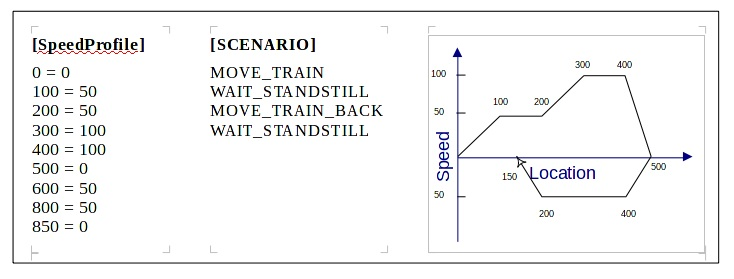
\includegraphics[width=\textwidth]{image/test_runner_speed_profile}
		\caption{Speed profile}
		\label{fig:Speed profile}
	\end{figure}
	\subsubsection{Balise section: BaliseTrackside}

	This section describes the locations at which balise messages have to be sent to the EVC (<location(m)> = <user balise message name>). A user defined section describing the balise message content is associated to each location. As for the speed profile, the locations are given for the travelled distance.
	
	The user defined sections contain the description of the balise message content. It uses the variable names as defined in SRS chapter 7 and 8 (See Erreur : source de la référence non trouvée) Message variables don’t need to be defined if the default value is used but they have to be in the right order.
	
	Note: The SRS language can be indicated in option with SRS=<version> Example: <location(m)> = <user balise message name>, SRS=2.3.0
	
	During the execution, balise message contents are automatically sent to EVC when the location is reached.
	
	The following example shows a balise trackside and the associated balise message content sections:
	
	\begin{tabular}{|l l l l l l|}
	
		\hline
		
		\multicolumn{2}{|l}{ \begin{minipage}[t]{0.33\linewidth} \textbf{[BaliseTrackside]} \end{minipage} } & \multicolumn{2}{l}{ \begin{minipage}[t]{0.33\linewidth} \textbf{[BG\_1\_0]} \end{minipage} } & \multicolumn{2}{l|}{ \begin{minipage}[t]{0.33\linewidth} \textbf{[BG\_1\_1]} \end{minipage} } \\ 
		100  &= BG\_1\_0 & \multicolumn{2}{l}{\emph{\# Header}} & \multicolumn{2}{l|}{\emph{\# Header}} \\ 
		105  &= BG\_1\_1 & N\_PIG &= 0 & N\_PIG &= 1 \\
		& & N\_TOTAL &= 1 & N\_TOTAL &= 1 \\
		& & NID\_C &= 0 & NID\_C &= 0 \\
		& & NID\_BG &= 1 & NID\_BG &= 1 \\
		& & Q\_LINK &= 1 & Q\_LINK &= 1 \\
		& & & & & \\
		& & \multicolumn{2}{l}{\emph{\# L1 MA packet}} & \multicolumn{2}{l|}{\emph{\# SSP packet}} \\ 
		& & NID\_PACKET &= 12 & NID\_PACKET &= 27 \\
		& & Q\_DIR &= 1 & Q\_DIR &= 2 \\
		& & Q\_SCALE &= 1 & V\_STATIC &= 2 \\
		& & V\_MAIN &= 30 & & \\
		& & L\_ENDSECTION &= 500 & \multicolumn{2}{l|}{\emph{\# Gradient packet}} \\ 
		& & & & NID\_PACKET &= 21 \\
		
		\hline
		
	\end{tabular}
	
\subsubsection{Loop  section: LoopTrackside}

	This section describes the locations at which loop messages have to be sent to the on-board (<location(m)> = <user loop message name>). A user defined section describing the loop message content is associated to each location. As for the speed profile, the locations are given for the travelled distance.
	
	The user defined sections contain the description of the loop message content. It uses the variable names as defined in SRS chapter 7 and 8 (See Erreur : source de la référence non trouvée for more details). Message variables don’t need to be defined if the default value is used but they have to be in the right order.
	
	Note:
	
	\begin{itemize}
		\item the SRS language can be indicated in option with SRS=<version>;
		\item the spread spectrum code value can be indicated in option with SSCode=<SSCode>, if not indicated default value 15 is used.
		\item Example: <location(m)> = <user loop message name>, SSCode=3, SRS=2.3.0
		
	\end{itemize} 
	
	During the execution, loop message contents are automatically sent to on-board when the location is reached.
	The following example shows a loop trackside and the associated loop message content sections:
	
	\begin{tabular}{|l l l l l l|}
	
		\hline
		
		\multicolumn{2}{|l}{ \begin{minipage}[t]{0.33\linewidth} \textbf{[LoopTrackside]} \end{minipage} } & \multicolumn{2}{l}{ \begin{minipage}[t]{0.33\linewidth} \textbf{[Loop0]} \end{minipage} } & \multicolumn{2}{l|}{ \begin{minipage}[t]{0.33\linewidth} \textbf{[Loop1]} \end{minipage} } \\ 
		100  &= Loop0 & \multicolumn{2}{l}{\emph{\# Header}} & \multicolumn{2}{l|}{\emph{\# Header}} \\ 
		105  &= Loop1 & NID\_C  &= 0 & NID\_C &= 0 \\
		& & NID\_LOOP  &= 1 & NID\_LOOP  &= 1 \\
		& & & & & \\
		& & \multicolumn{2}{l}{\emph{\# Infill location reference}} & \multicolumn{2}{l|}{\emph{\# Infill location reference}} \\ 
		& & NID\_PACKET &= 136 & NID\_PACKET &= 136 \\
		& & Q\_DIR &= 2 & Q\_DIR &= 2 \\
		& & NID\_BG &= 1 & NID\_BG &= 1 \\
		& & & & & \\
		& & \multicolumn{2}{l}{\emph{\# L1 MA packet}} & \multicolumn{2}{l|}{\emph{\# L1 MA packet}}  \\
		& & NID\_PACKET &= 12 & NID\_PACKET &= 12 \\
		& & Q\_DIR &= 2 & Q\_DIR &= 2 \\
		& & Q\_SCALE &= 1 & Q\_SCALE &= 1 \\
		& & V\_MAIN	&= 0 & V\_MAIN &= 30 \\
		& & L\_ENDSECTION &= 0 & L\_ENDSECTION &= 500 \\
		& & & & & \\
		& & \multicolumn{2}{l}{\emph{\# SSP packet}} & \multicolumn{2}{l|}{\emph{\# SSP packet}}  \\
		& & NID\_PACKET &= 27 & NID\_PACKET &= 27 \\
		& & Q\_DIR &= 2 & Q\_DIR &= 2 \\
		& & V\_STATIC &= 30 & V\_STATIC &= 30 \\
		& & & & & \\
		& & \multicolumn{2}{l}{\emph{\# Gradient packet}} & \multicolumn{2}{l|}{\emph{\# Gradient packet}}  \\
		& & NID\_PACKET &= 21 & NID\_PACKET &= 21 \\ 
		
		\hline
		
	\end{tabular}

\subsubsection{Default national values configuration section: Config\_SRSNationalDefaults}
	This section defines the default national values used by EVC, before Start-of-Mission. These default national values can be overridden when the train receives a packet 3 from trackside. This will allow the Test Environment to be able to test the correct update of the national values data.
	
	\begin{itemize}
		\item COUNTRY\_ID:
		
			\begin{longtable}{|l|l|}
				\caption{COUNTRY\_ID}\\ 
				\hline
				
					\begin{minipage}[t]{0.22\linewidth} \textbf{Description}	\end{minipage} 
				&	\begin{minipage}[t]{0.78\linewidth} Country identifier of the country for which default national values are valid. \end{minipage} \\
				
				\hline
				
					\begin{minipage}[t]{0.22\linewidth} \textbf{Default value}	\end{minipage} 
				&	\begin{minipage}[t]{0.78\linewidth} 0 \end{minipage} \\
				
				\hline
				
			\end{longtable}
			
		\item COUNTRIES\_ID:
		
			\begin{longtable}{|l|l|}
				\caption{COUNTRIES\_ID}\\ 
				\hline
				
					\begin{minipage}[t]{0.22\linewidth} \textbf{Description}	\end{minipage} 
				&	\begin{minipage}[t]{0.78\linewidth} A list of country identifiers for which default national values are valid. \end{minipage} \\
				
				\hline
				
					\begin{minipage}[t]{0.22\linewidth} \textbf{Default value}	\end{minipage} 
				&	\begin{minipage}[t]{0.78\linewidth} 0 \end{minipage} \\
				
				\hline
				
					\begin{minipage}[t]{0.22\linewidth} \textbf{Example}	\end{minipage} 
				&	\begin{minipage}[t]{0.78\linewidth} COUNTRIES\_ID = 253;254 \end{minipage} \\
				
				\hline
				
			\end{longtable}			
			
		\item DRIVER\_ADHESION:
		
			\begin{longtable}{|l|l|}
				\caption{DRIVER\_ADHESION}\\ 	
				\hline
				
					\begin{minipage}[t]{0.22\linewidth} \textbf{Description}	\end{minipage} 
				&	\begin{minipage}[t]{0.78\linewidth} Qualifier for the modification of trackside adhesion factor by driver. \end{minipage} \\
				
				\hline
				
					\begin{minipage}[t]{0.22\linewidth} \textbf{SRS Name}	\end{minipage} 
				&	\begin{minipage}[t]{0.78\linewidth} \emph{\texttt{Q\_NVDRIVER\_ADHES}} \end{minipage} \\
				
				\hline
														
					\begin{minipage}[t]{0.22\linewidth} \textbf{Special values}	\end{minipage} 
				&	\begin{minipage}[t]{0.78\linewidth} \begin{itemize} \item 0: not allowed \item 1: allowed \end{itemize} \end{minipage} \\
				
				\hline
										
					\begin{minipage}[t]{0.22\linewidth} \textbf{Default value}	\end{minipage} 
				&	\begin{minipage}[t]{0.78\linewidth} 0 \end{minipage} \\
				
				\hline
				
			\end{longtable}
			
			
		\item SH\_SPEED:
			\begin{longtable}{|l|l|}
				\caption{SH\_SPEED}\\ 				
				\hline
				
					\begin{minipage}[t]{0.22\linewidth} \textbf{Description}	\end{minipage} 
				&	\begin{minipage}[t]{0.78\linewidth} Shunting mode permitted speed (km/h). \end{minipage} \\
				
				\hline
				
					\begin{minipage}[t]{0.22\linewidth} \textbf{SRS Name}	\end{minipage} 
				&	\begin{minipage}[t]{0.78\linewidth} \emph{\texttt{V\_NVSHUNT}} \end{minipage} \\
				
				\hline
														
					\begin{minipage}[t]{0.22\linewidth} \textbf{Range}	\end{minipage} 
				&	\begin{minipage}[t]{0.78\linewidth} 0 km/h – 600 km/h (in 5 km/h step) \end{minipage} \\
				
				\hline
										
					\begin{minipage}[t]{0.22\linewidth} \textbf{Default value}	\end{minipage} 
				&	\begin{minipage}[t]{0.78\linewidth} 30 km/h \end{minipage} \\
				
				\hline
				
			\end{longtable}
			
			
		\item SR\_SPEED:
			\begin{longtable}{|l|l|}
				\caption{SR\_SPEED}\\ 							
				\hline
				
					\begin{minipage}[t]{0.22\linewidth} \textbf{Description}	\end{minipage} 
				&	\begin{minipage}[t]{0.78\linewidth} Staff Responsible mode permitted speed (km/h). \end{minipage} \\
				
				\hline
				
					\begin{minipage}[t]{0.22\linewidth} \textbf{SRS Name}	\end{minipage} 
				&	\begin{minipage}[t]{0.78\linewidth} \emph{\texttt{V\_NVSTFF}} \end{minipage} \\
				
				\hline
														
					\begin{minipage}[t]{0.22\linewidth} \textbf{Range}	\end{minipage} 
				&	\begin{minipage}[t]{0.78\linewidth} 0 km/h – 600 km/h (in 5 km/h step) \end{minipage} \\
				
				\hline
										
					\begin{minipage}[t]{0.22\linewidth} \textbf{Default value}	\end{minipage} 
				&	\begin{minipage}[t]{0.78\linewidth} 40 km/h \end{minipage} \\
				
				\hline
				
			\end{longtable}
			
			
		\item OS\_SPEED:
		
			\begin{longtable}{|l|l|}
				\caption{OS\_SPEED}\\ 							
				\hline
				
					\begin{minipage}[t]{0.22\linewidth} \textbf{Description}	\end{minipage} 
				&	\begin{minipage}[t]{0.78\linewidth} On Sight mode permitted speed (km/h). \end{minipage} \\
				
				\hline
				
					\begin{minipage}[t]{0.22\linewidth} \textbf{SRS Name}	\end{minipage} 
				&	\begin{minipage}[t]{0.78\linewidth} \emph{\texttt{V\_NVONSIGHT}} \end{minipage} \\
				
				\hline
														
					\begin{minipage}[t]{0.22\linewidth} \textbf{Range}	\end{minipage} 
				&	\begin{minipage}[t]{0.78\linewidth} 0 km/h – 600 km/h (in 5 km/h step) \end{minipage} \\
				
				\hline
										
					\begin{minipage}[t]{0.22\linewidth} \textbf{Default value}	\end{minipage} 
				&	\begin{minipage}[t]{0.78\linewidth} 30 km/h \end{minipage} \\
				
				\hline
				
			\end{longtable}			 
			
		\item UN\_SPEED:
			\begin{longtable}{|l|l|}
				\caption{UN\_SPEED}\\ 										
				\hline
				
					\begin{minipage}[t]{0.22\linewidth} \textbf{Description}	\end{minipage} 
				&	\begin{minipage}[t]{0.78\linewidth} Unfitted mode permitted speed (km/h). \end{minipage} \\
				
				\hline
				
					\begin{minipage}[t]{0.22\linewidth} \textbf{SRS Name}	\end{minipage} 
				&	\begin{minipage}[t]{0.78\linewidth} \emph{\texttt{V\_NVUNFIT}} \end{minipage} \\
				
				\hline
														
					\begin{minipage}[t]{0.22\linewidth} \textbf{Range}	\end{minipage} 
				&	\begin{minipage}[t]{0.78\linewidth} 0 km/h – 600 km/h (in 5 km/h step) \end{minipage} \\
				
				\hline
										
					\begin{minipage}[t]{0.22\linewidth} \textbf{Default value}	\end{minipage} 
				&	\begin{minipage}[t]{0.78\linewidth} 100 km/h \end{minipage} \\
				
				\hline
				
			\end{longtable}
						
			
			
		\item RELEASE\_SPEED:
		
			\begin{longtable}{|l|l|}
				\caption{RELEASE\_SPEED}\\ 												
				\hline
				
					\begin{minipage}[t]{0.22\linewidth} \textbf{Description}	\end{minipage} 
				&	\begin{minipage}[t]{0.78\linewidth} Release Speed permitted speed (km/h). \end{minipage} \\
				
				\hline
				
					\begin{minipage}[t]{0.22\linewidth} \textbf{SRS Name}	\end{minipage} 
				&	\begin{minipage}[t]{0.78\linewidth} \emph{\texttt{V\_NVREL}} \end{minipage} \\
				
				\hline
														
					\begin{minipage}[t]{0.22\linewidth} \textbf{Range}	\end{minipage} 
				&	\begin{minipage}[t]{0.78\linewidth} 0 km/h – 600 km/h (in 5 km/h step) \end{minipage} \\
				
				\hline
										
					\begin{minipage}[t]{0.22\linewidth} \textbf{Default value}	\end{minipage} 
				&	\begin{minipage}[t]{0.78\linewidth} 40 km/h \end{minipage} \\
				
				\hline
				
			\end{longtable}						
			
		\item ROLLAWAY\_DISTANCE:
		
			\begin{longtable}{|l|l|}
				\caption{ROLLAWAY\_DISTANCE}\\ 														
				\hline
				
					\begin{minipage}[t]{0.22\linewidth} \textbf{Description}	\end{minipage} 
				&	\begin{minipage}[t]{0.78\linewidth} Distance limit used for roll away and reverse movement protection (meter). \end{minipage} \\
				
				\hline
				
					\begin{minipage}[t]{0.22\linewidth} \textbf{SRS Name}	\end{minipage} 
				&	\begin{minipage}[t]{0.78\linewidth} \emph{\texttt{D\_NVROLL}} \end{minipage} \\
				
				\hline
														
					\begin{minipage}[t]{0.22\linewidth} \textbf{Range}	\end{minipage} 
				&	\begin{minipage}[t]{0.78\linewidth} 0 meters – 327 660 meters (in 1 meter step) \end{minipage} \\
				
				\hline
																		
					\begin{minipage}[t]{0.22\linewidth} \textbf{Special values}	\end{minipage} 
				&	\begin{minipage}[t]{0.78\linewidth} INFINITY: deactivates roll away and reverse movement protection \end{minipage} \\
								
				\hline
										
					\begin{minipage}[t]{0.22\linewidth} \textbf{Default value}	\end{minipage} 
				&	\begin{minipage}[t]{0.78\linewidth} 2 meters \end{minipage} \\
				
				\hline
				
			\end{longtable}
			
			
		\item SB\_USETOTARGET:
		
			\begin{longtable}{|l|l|}
				\caption{SB\_USETOTARGET}\\ 																	
				\hline
				
					\begin{minipage}[t]{0.22\linewidth} \textbf{Description}	\end{minipage} 
				&	\begin{minipage}[t]{0.78\linewidth} Permission to use service brake when braking to a target is supervised. \end{minipage} \\
				
				\hline
				
					\begin{minipage}[t]{0.22\linewidth} \textbf{SRS Name}	\end{minipage} 
				&	\begin{minipage}[t]{0.78\linewidth} \emph{\texttt{Q\_NVSRBKTRG}} \end{minipage} \\
				
				\hline
																																
					\begin{minipage}[t]{0.22\linewidth} \textbf{Special values}	\end{minipage} 
				&	\begin{minipage}[t]{0.78\linewidth} \begin{itemize} \item 0: no \item 1: yes \end{itemize} \end{minipage} \\
								
				\hline
										
					\begin{minipage}[t]{0.22\linewidth} \textbf{Default value}	\end{minipage} 
				&	\begin{minipage}[t]{0.78\linewidth} yes \end{minipage} \\
				
				\hline
				
			\end{longtable}
			
		\item EB\_RUNRELEASE:
		
			\begin{longtable}{|l|l|}
				\caption{EB\_RUNRELEASE}\\ 																	
				\hline
				
					\begin{minipage}[t]{0.22\linewidth} \textbf{Description}	\end{minipage} 
				&	\begin{minipage}[t]{0.78\linewidth} Permission to release the emergency brake immediately if the condition why the system has triggered the emergency brake (speed exceeds emergency brake intervention limit, lack of driver reaction) is not fulfilled any more. \end{minipage} \\
				
				\hline
				
					\begin{minipage}[t]{0.22\linewidth} \textbf{SRS Name}	\end{minipage} 
				&	\begin{minipage}[t]{0.78\linewidth} \emph{\texttt{Q\_NVEMRRLS}} \end{minipage} \\
				
				\hline
																																
					\begin{minipage}[t]{0.22\linewidth} \textbf{Special values}	\end{minipage} 
				&	\begin{minipage}[t]{0.78\linewidth} \begin{itemize} \item 0: only at standstill \item 1: immediate release possible \end{itemize} \end{minipage} \\
								
				\hline
										
					\begin{minipage}[t]{0.22\linewidth} \textbf{Default value}	\end{minipage} 
				&	\begin{minipage}[t]{0.78\linewidth} only at standstill \end{minipage} \\
				
				\hline
				
			\end{longtable}
		\item OVERRIDEEOA\_ENTRYSPEED:
		
			\begin{longtable}{|l|l|}
				\caption{OVERRIDEEOA\_ENTRYSPEED}\\ 																	
				\hline
				
					\begin{minipage}[t]{0.22\linewidth} \textbf{Description}	\end{minipage} 
				&	\begin{minipage}[t]{0.78\linewidth} Maximum speed limit allowing the driver to select the ”override EOA” function (km/h). \end{minipage} \\
				
				\hline
				
					\begin{minipage}[t]{0.22\linewidth} \textbf{SRS Name}	\end{minipage} 
				&	\begin{minipage}[t]{0.78\linewidth} \emph{\texttt{V\_NVALLOWOVTRP}} \end{minipage} \\
				
				\hline
																																
					\begin{minipage}[t]{0.22\linewidth} \textbf{Range}	\end{minipage} 
				&	\begin{minipage}[t]{0.78\linewidth} 0 km/h – 600 km/h (in 5 km/h step) \end{minipage} \\
								
				\hline
										
					\begin{minipage}[t]{0.22\linewidth} \textbf{Default value}	\end{minipage} 
				&	\begin{minipage}[t]{0.78\linewidth} 0 km/h \end{minipage} \\
				
				\hline
				
			\end{longtable}
			
		\item OVERRIDEEOA\_MAXSPEED:
		
			\begin{longtable}{|l|l|}
				\caption{OVERRIDEEOA\_MAXSPEED}\\ 																				
				\hline
				
					\begin{minipage}[t]{0.22\linewidth} \textbf{Description}	\end{minipage} 
				&	\begin{minipage}[t]{0.78\linewidth} Permitted speed limit to be supervised when the ”override EOA” function is active (km/h). \end{minipage} \\
				
				\hline
				
					\begin{minipage}[t]{0.22\linewidth} \textbf{SRS Name}	\end{minipage} 
				&	\begin{minipage}[t]{0.78\linewidth} \emph{\texttt{V\_NVSUPOVTRP}} \end{minipage} \\
				
				\hline
																																
					\begin{minipage}[t]{0.22\linewidth} \textbf{Range}	\end{minipage} 
				&	\begin{minipage}[t]{0.78\linewidth} 0 km/h – 600 km/h (in 5 km/h step) \end{minipage} \\
								
				\hline
										
					\begin{minipage}[t]{0.22\linewidth} \textbf{Default value}	\end{minipage} 
				&	\begin{minipage}[t]{0.78\linewidth} 30 km/h \end{minipage} \\
				
				\hline
				
			\end{longtable}
					
		\item OVERRIDEEOA\_MAXDISTANCE:
		
			\begin{longtable}{|l|l|}
				\caption{OVERRIDEEOA\_MAXDISTANCE}\\ 																						
				\hline
				
					\begin{minipage}[t]{0.22\linewidth} \textbf{Description}	\end{minipage} 
				&	\begin{minipage}[t]{0.78\linewidth} Maximum distance for overriding the train trip (meter). \end{minipage} \\
				
				\hline
				
					\begin{minipage}[t]{0.22\linewidth} \textbf{SRS Name}	\end{minipage} 
				&	\begin{minipage}[t]{0.78\linewidth} \emph{\texttt{D\_NVOVTRP}} \end{minipage} \\
				
				\hline
																																
					\begin{minipage}[t]{0.22\linewidth} \textbf{Range}	\end{minipage} 
				&	\begin{minipage}[t]{0.78\linewidth} 0 meters – 327 670 meters (in 1 meter step) \end{minipage} \\
								
				\hline
										
					\begin{minipage}[t]{0.22\linewidth} \textbf{Default value}	\end{minipage} 
				&	\begin{minipage}[t]{0.78\linewidth} 200 meters \end{minipage} \\
				
				\hline
				
			\end{longtable}
			
			
		\item OVERRIDEEOA\_MAXTIME:
		
			\begin{longtable}{|l|l|}
				\caption{OVERRIDEEOA\_MAXTIME}\\ 																									
				\hline
				
					\begin{minipage}[t]{0.22\linewidth} \textbf{Description}	\end{minipage} 
				&	\begin{minipage}[t]{0.78\linewidth} Maximum time for overriding the train trip (second). \end{minipage} \\
				
				\hline
																																				
					\begin{minipage}[t]{0.22\linewidth} \textbf{Range}	\end{minipage} 
				&	\begin{minipage}[t]{0.78\linewidth} 0 second – 255 seconds (in 1 second step) \end{minipage} \\
								
				\hline
										
					\begin{minipage}[t]{0.22\linewidth} \textbf{Default value}	\end{minipage} 
				&	\begin{minipage}[t]{0.78\linewidth} 60 seconds \end{minipage} \\
				
				\hline
				
			\end{longtable}
					
		\item DRIVERID\_RUNCHANGE:
		
			\begin{longtable}{|l|l|}
				\caption{DRIVERID\_RUNCHANGE}\\ 																				
				\hline
				
					\begin{minipage}[t]{0.22\linewidth} \textbf{Description}	\end{minipage} 
				&	\begin{minipage}[t]{0.78\linewidth} Entry of Driver ID permitted while running. \end{minipage} \\
				
				\hline
				
					\begin{minipage}[t]{0.22\linewidth} \textbf{SRS Name}	\end{minipage} 
				&	\begin{minipage}[t]{0.78\linewidth} \emph{\texttt{M\_NVDERUN}} \end{minipage} \\
				
				\hline
																																
					\begin{minipage}[t]{0.22\linewidth} \textbf{Special values}	\end{minipage} 
				&	\begin{minipage}[t]{0.78\linewidth} \begin{itemize} \item 0: no \item 1: yes \end{itemize} \end{minipage} \\
								
				\hline
										
					\begin{minipage}[t]{0.22\linewidth} \textbf{Default value}	\end{minipage} 
				&	\begin{minipage}[t]{0.78\linewidth} yes \end{minipage} \\
				
				\hline
				
			\end{longtable}
								
		\item PT\_MAXDISTANCE:
		
			\begin{longtable}{|l|l|}
				\caption{PT\_MAXDISTANCE}\\ 																							
				\hline
				
					\begin{minipage}[t]{0.22\linewidth} \textbf{Description}	\end{minipage} 
				&	\begin{minipage}[t]{0.78\linewidth} Maximum distance for reversing in Post Trip mode (meter). \end{minipage} \\
				
				\hline
				
					\begin{minipage}[t]{0.22\linewidth} \textbf{SRS Name}	\end{minipage} 
				&	\begin{minipage}[t]{0.78\linewidth} \emph{\texttt{D\_NVPOTRP}} \end{minipage} \\
				
				\hline
																																
					\begin{minipage}[t]{0.22\linewidth} \textbf{Range}	\end{minipage} 
				&	\begin{minipage}[t]{0.78\linewidth} 0 meters – 327 670 meters (in 1 meter step) \end{minipage} \\
								
				\hline
										
					\begin{minipage}[t]{0.22\linewidth} \textbf{Default value}	\end{minipage} 
				&	\begin{minipage}[t]{0.78\linewidth} 200 meters \end{minipage} \\
				
				\hline
				
			\end{longtable}
			
		\item CONTACT\_TIME:
		
			\begin{longtable}{|l|l|}
				\caption{CONTACT\_TIME}\\ 																										
				\hline
				
					\begin{minipage}[t]{0.22\linewidth} \textbf{Description}	\end{minipage} 
				&	\begin{minipage}[t]{0.78\linewidth} Maximal time without new ”safe” radio message (second). \end{minipage} \\
				
				\hline
				
					\begin{minipage}[t]{0.22\linewidth} \textbf{SRS Name}	\end{minipage} 
				&	\begin{minipage}[t]{0.78\linewidth} \emph{\texttt{T\_NVCONTACT}} \end{minipage} \\
				
				\hline
																																
					\begin{minipage}[t]{0.22\linewidth} \textbf{Range}	\end{minipage} 
				&	\begin{minipage}[t]{0.78\linewidth} 0 second – 254 seconds (in 1 second step) \end{minipage} \\
					
				\hline
																																					
					\begin{minipage}[t]{0.22\linewidth} \textbf{Special values}	\end{minipage} 
				&	\begin{minipage}[t]{0.78\linewidth} INFINITY: deactivates supervision of radio link \end{minipage} \\	
						
				\hline
										
					\begin{minipage}[t]{0.22\linewidth} \textbf{Default value}	\end{minipage} 
				&	\begin{minipage}[t]{0.78\linewidth} ∞ seconds \end{minipage} \\
				
				\hline
				
			\end{longtable}
				
		\item SR\_MAXDISTANCE:
		
			\begin{longtable}{|l|l|}
				\caption{SR\_MAXDISTANCE}\\ 																													
				\hline
				
					\begin{minipage}[t]{0.22\linewidth} \textbf{Description}	\end{minipage} 
				&	\begin{minipage}[t]{0.78\linewidth} Maximum distance for running in Staff Responsible mode (meter). \end{minipage} \\
				
				\hline
				
					\begin{minipage}[t]{0.22\linewidth} \textbf{SRS Name}	\end{minipage} 
				&	\begin{minipage}[t]{0.78\linewidth} \emph{\texttt{D\_NVSTFF}} \end{minipage} \\
				
				\hline
																																
					\begin{minipage}[t]{0.22\linewidth} \textbf{Range}	\end{minipage} 
				&	\begin{minipage}[t]{0.78\linewidth} 0 meters – 327 660 meters (in 1 meter step) \end{minipage} \\
					
				\hline
																																					
					\begin{minipage}[t]{0.22\linewidth} \textbf{Special values}	\end{minipage} 
				&	\begin{minipage}[t]{0.78\linewidth} INFINITY: deactivates distance supervision in Staff Responsible mode \end{minipage} \\	
						
				\hline
										
					\begin{minipage}[t]{0.22\linewidth} \textbf{Default value}	\end{minipage} 
				&	\begin{minipage}[t]{0.78\linewidth} ∞ meters \end{minipage} \\
				
				\hline
				
			\end{longtable}
			
		\item NOCONTACT\_REACTION:
		
			\begin{longtable}{|l|l|}
				\caption{NOCONTACT\_REACTION}\\ 																																
				\hline
				
					\begin{minipage}[t]{0.22\linewidth} \textbf{Description}	\end{minipage} 
				&	\begin{minipage}[t]{0.78\linewidth} Indicates the reaction to be performed when T\_NVCONTACT timer elapses. \end{minipage} \\
				
				\hline
				
					\begin{minipage}[t]{0.22\linewidth} \textbf{SRS Name}	\end{minipage} 
				&	\begin{minipage}[t]{0.78\linewidth} \emph{\texttt{M\_NVCONTACT}} \end{minipage} \\
				
				\hline
																																									
					\begin{minipage}[t]{0.22\linewidth} \textbf{Special values}	\end{minipage} 
				&	\begin{minipage}[t]{0.78\linewidth} \begin{itemize} \item NONE: no reaction \item TRIP: train trip \item SB: service brake application \end{itemize} \end{minipage} \\	
						
				\hline
										
					\begin{minipage}[t]{0.22\linewidth} \textbf{Default value}	\end{minipage} 
				&	\begin{minipage}[t]{0.78\linewidth} no reaction \end{minipage} \\
				
				\hline
				
			\end{longtable}
			
		\item NV\_FROM\_HEX\_BUFFER:
		
			\begin{longtable}{|l|l|}
				\caption{NV\_FROM\_HEX\_BUFFER}\\ 																																
				\hline
				
					\begin{minipage}[t]{0.22\linewidth} \textbf{Description}	\end{minipage} 
				&	\begin{minipage}[t]{0.78\linewidth} Allows to initialize EVC with a general radio message (24) containing packet 3. \end{minipage} \\
				
				\hline
				
					\begin{minipage}[t]{0.22\linewidth} \textbf{Format}	\end{minipage} 
				&	\begin{minipage}[t]{0.78\linewidth}A list of hexadecimal values splited by comma that represents general radio message\end{minipage} \\
				
				\hline
																																									
					\begin{minipage}[t]{0.22\linewidth} \textbf{Example}	\end{minipage} 
				&	\begin{minipage}[t]{0.78\linewidth} NV\_FROM\_HEX\_BUFFER = 18, 08, 80, 00, 00, 00, 00, 00, 00, 00, 68, 31, 10, 00, 02, 3f, 4f, f0, c1, 83, 20, 0a, 00, 28, 06, 18, 03, 27, f8, 0c, 84, 69, ff, fd \end{minipage} \\	
						
				\hline
										
					\begin{minipage}[t]{0.22\linewidth} \textbf{Default value}	\end{minipage} 
				&	\begin{minipage}[t]{0.78\linewidth} none \end{minipage} \\
				
				\hline
					\begin{minipage}[t]{0.22\linewidth} \textbf{Warning}	\end{minipage} 
				&	\begin{minipage}[t]{0.78\linewidth} If NV\_FROM\_HEX\_BUFFER is defined all other values define in this section are removed\end{minipage} \\
				
				\hline
				
			\end{longtable}
		
	\end{itemize}
	
\subsubsection{EVC configuration section: Config\_EVCInit}
This section allow definition of values of the EVC at power on, i.e. at initialization state.
	\begin{itemize}
		\item LINE\_LEVEL:
		
			\begin{longtable}{|l|l|}
				\caption{LINE\_LEVEL}\\ 
				\hline
				
					\begin{minipage}[t]{0.22\linewidth} \textbf{Description}	\end{minipage} 
				&	\begin{minipage}[t]{0.78\linewidth} Default ETCS level. \end{minipage} \\
				
				\hline
																																									
					\begin{minipage}[t]{0.22\linewidth} \textbf{Special values}	\end{minipage} 
				&	\begin{minipage}[t]{0.78\linewidth} \begin{itemize} \item 0: level 0 \item 1: level 1 \item 2: level 2 \item 3: level 3 \end{itemize} \end{minipage} \\
				
				\hline
				
					\begin{minipage}[t]{0.22\linewidth} \textbf{Default value}	\end{minipage} 
				&	\begin{minipage}[t]{0.78\linewidth} level 3 \end{minipage} \\
				
				\hline
				
			\end{longtable}
			
		\item RBC\_ID:
				
			\begin{longtable}{|l|l|}
				\caption{RBC\_ID}\\ 
				\hline
				
					\begin{minipage}[t]{0.22\linewidth} \textbf{Description}	\end{minipage} 
				&	\begin{minipage}[t]{0.78\linewidth} Default RBC identifier. \end{minipage} \\
				
				\hline
																																									
					\begin{minipage}[t]{0.22\linewidth} \textbf{Range}	\end{minipage} 
				&	\begin{minipage}[t]{0.78\linewidth} \[ RBC\_ID = NID\_C * 2^{14} + NID\_RBC \] \begin{itemize} \item NID\_C: 0 – 1024 \item NID\_RBC: 0 – 16384 \end{itemize} \end{minipage} \\
				
				\hline
				
					\begin{minipage}[t]{0.22\linewidth} \textbf{Default value}	\end{minipage} 
				&	\begin{minipage}[t]{0.78\linewidth} 789 \end{minipage} \\
				
				\hline
				
			\end{longtable}
			
		\item RBC\_PHONE:
						
			\begin{longtable}{|l|l|}
				\caption{RBC\_PHONE}\\ 
				\hline
				
					\begin{minipage}[t]{0.22\linewidth} \textbf{Description}	\end{minipage} 
				&	\begin{minipage}[t]{0.78\linewidth} Default RBC phone number. \end{minipage} \\
				
				\hline
																																									
					\begin{minipage}[t]{0.22\linewidth} \textbf{Range}	\end{minipage} 
				&	\begin{minipage}[t]{0.78\linewidth} 1 to 16 digits value \end{minipage} \\
				
				\hline
				
					\begin{minipage}[t]{0.22\linewidth} \textbf{Default value}	\end{minipage} 
				&	\begin{minipage}[t]{0.78\linewidth} 1234123412341234 \end{minipage} \\
				
				\hline
				
			\end{longtable}
			
		\item NETWORK\_ID:
								
			\begin{longtable}{|l|l|}
				\caption{NETWORK\_ID}\\ 
				\hline
				
					\begin{minipage}[t]{0.22\linewidth} \textbf{Description}	\end{minipage} 
				&	\begin{minipage}[t]{0.78\linewidth} Default radio network identifier. \end{minipage} \\
				
				\hline
																																									
					\begin{minipage}[t]{0.22\linewidth} \textbf{Range}	\end{minipage} 
				&	\begin{minipage}[t]{0.78\linewidth} 1 to 6 digits value \end{minipage} \\
				
				\hline
				
					\begin{minipage}[t]{0.22\linewidth} \textbf{Default value}	\end{minipage} 
				&	\begin{minipage}[t]{0.78\linewidth} 123456 \end{minipage} \\
				
				\hline
				
			\end{longtable}
			
		\item COUNTRY\_ID:
										
			\begin{longtable}{|l|l|}
				\caption{COUNTRY\_ID}\\ 
				\hline
				
					\begin{minipage}[t]{0.22\linewidth} \textbf{Description} \end{minipage} 
				&	\begin{minipage}[t]{0.78\linewidth} Country identifier of the last relevant balise group (LRBG). \end{minipage} \\
				
				\hline
																																									
					\begin{minipage}[t]{0.22\linewidth} \textbf{Range} \end{minipage} 
				&	\begin{minipage}[t]{0.78\linewidth} 0 – 1024 \end{minipage} \\
				
				\hline
				
					\begin{minipage}[t]{0.22\linewidth} \textbf{Default value} \end{minipage} 
				&	\begin{minipage}[t]{0.78\linewidth} 0 \end{minipage} \\
				
				\hline
				
			\end{longtable}
			
		\item GROUP\_ID:
												
			\begin{longtable}{|l|l|}
				\caption{GROUP\_ID}\\ 
				\hline
				
					\begin{minipage}[t]{0.22\linewidth} \textbf{Description} \end{minipage} 
				&	\begin{minipage}[t]{0.78\linewidth} Identifier of the last relevant balise group (LRBG). \end{minipage} \\
				
				\hline
																																									
					\begin{minipage}[t]{0.22\linewidth} \textbf{Range} \end{minipage} 
				&	\begin{minipage}[t]{0.78\linewidth} 0 – 16384 \end{minipage} \\
				
				\hline
				
					\begin{minipage}[t]{0.22\linewidth} \textbf{Default value} \end{minipage} 
				&	\begin{minipage}[t]{0.78\linewidth} 4522 \end{minipage} \\
				
				\hline
				
			\end{longtable}
			
		\item DISTANCE:
													
			\begin{longtable}{|l|l|}
				\caption{DISTANCE}\\ 
				\hline
				
					\begin{minipage}[t]{0.22\linewidth} \textbf{Description} \end{minipage} 
				&	\begin{minipage}[t]{0.78\linewidth} Distance to the reference last relevant balise group from train front. \end{minipage} \\
				
				\hline
																																									
					\begin{minipage}[t]{0.22\linewidth} \textbf{Range}	\end{minipage} 
				&	\begin{minipage}[t]{0.78\linewidth} 0 meter – 327 670 meters \end{minipage} \\
				
				\hline
				
					\begin{minipage}[t]{0.22\linewidth} \textbf{Default value}	\end{minipage} 
				&	\begin{minipage}[t]{0.78\linewidth} 50 \end{minipage} \\
				
				\hline
				
			\end{longtable}
		
		\item DIRECTION:
															
			\begin{longtable}{|l|l|}
				\caption{DIRECTION}\\ 
				\hline
				
					\begin{minipage}[t]{0.22\linewidth} \textbf{Description} \end{minipage} 
				&	\begin{minipage}[t]{0.78\linewidth} Validity direction for the reference balise group (LRBG). \end{minipage} \\
				
				\hline
																																									
					\begin{minipage}[t]{0.22\linewidth} \textbf{Special values}	\end{minipage} 
				&	\begin{minipage}[t]{0.78\linewidth} \begin{itemize} \item NOMINAL \item REVERSE \item UNDEFINED \end{itemize} \end{minipage} \\
				
				\hline
				
					\begin{minipage}[t]{0.22\linewidth} \textbf{Default value}	\end{minipage} 
				&	\begin{minipage}[t]{0.78\linewidth} NOMINAL \end{minipage} \\
				
				\hline
				
			\end{longtable}
		
		\item VALIDITY:
																	
			\begin{longtable}{|l|l|}
				\caption{VALIDITY}\\ 
				\hline
				
					\begin{minipage}[t]{0.22\linewidth} \textbf{Description} \end{minipage} 
				&	\begin{minipage}[t]{0.78\linewidth} Validity of the last relevant balise group (LRBG). \end{minipage} \\
				
				\hline
																																									
					\begin{minipage}[t]{0.22\linewidth} \textbf{Special values}	\end{minipage} 
				&	\begin{minipage}[t]{0.78\linewidth} \begin{itemize} \item VALID \item INVALID \item UNKNOWN \end{itemize} \end{minipage} \\
				
				\hline
				
					\begin{minipage}[t]{0.22\linewidth} \textbf{Default value}	\end{minipage} 
				&	\begin{minipage}[t]{0.78\linewidth} VALID \end{minipage} \\
				
				\hline
				
			\end{longtable}
			
		\item NTC\_MODULE:
																			
			\begin{longtable}{|l|l|}
				\caption{NTC\_MODULE}\\ 
				\hline
				
					\begin{minipage}[t]{0.22\linewidth} \textbf{Description} \end{minipage} 
				&	\begin{minipage}[t]{0.78\linewidth} Name of the NTC module to instantiate (only one currently). \end{minipage} \\
				
				\hline
																																									
					\begin{minipage}[t]{0.22\linewidth} \textbf{Special values}	\end{minipage} 
				&	\begin{minipage}[t]{0.78\linewidth} \begin{itemize} \item GENERIC \item GENERICSS \item TEST \end{itemize} \end{minipage} \\
				
				\hline
				
					\begin{minipage}[t]{0.22\linewidth} \textbf{Default value}	\end{minipage} 
				&	\begin{minipage}[t]{0.78\linewidth} GENERIC \end{minipage} \\
				
				\hline
				
			\end{longtable}
			
		\item EVC\_CONFIG:
																			
			\begin{longtable}{|l|l|}
				\caption{EVC\_CONFIG}\\ 
				\hline
				
					\begin{minipage}[t]{0.22\linewidth} \textbf{Description} \end{minipage} 
				&	\begin{minipage}[t]{0.78\linewidth} Allows to activate EVC configuration. \end{minipage} \\
				
				\hline
																																									
					\begin{minipage}[t]{0.22\linewidth} \textbf{Values}	\end{minipage} 
				&	\begin{minipage}[t]{0.78\linewidth} \begin{itemize} 
																								\item CFG\_RADIO\_INTERNAL\_TIME\_STAMP : Internal time stamping (not use T\_TRAIN)
																								\item CFG\_USE\_JRU : Use JRU (generates JRU data file)
																								\item CFG\_RECORD\_TO\_CSV\_FILE : Record supervision data to CSV file
																								\item CFG\_BAL\_WITH\_ODO\_STAMP : Balise are received with odo stamp
																								\item CFG\_LOOP\_WITH\_SSCODE : Loop are received with spread spectrum code
																								\item CFG\_LOCAL\_TIME\_STAMP : Request local time stamp otherwise GMT time in log \& JRU record
																								\item CFG\_RECORDER\_LOG\_ADD\_FULL\_TIME\_STAMP : add time stamp in EuroCabLog.dat like 2009-05-29/08:15:21.29
																							\end{itemize} 
					\end{minipage} \\
				
				\hline
				
					\begin{minipage}[t]{0.22\linewidth} \textbf{Example}	\end{minipage} 
				&	\begin{minipage}[t]{0.78\linewidth} EVC\_CONFIG = CFG\_LOOP\_WITH\_SSCODE|CFG\_USE\_JRU \end{minipage} \\
				
				\hline
			
					\begin{minipage}[t]{0.22\linewidth} \textbf{Warning}	\end{minipage} 
				&	\begin{minipage}[t]{0.78\linewidth} CFG\_RADIO\_INTERNAL\_TIME\_STAMP and CFG\_BAL\_WITH\_ODO\_STAMP are mandatories for EVC then EVC set these configurations automatically and they can be removed\end{minipage} \\
				
				\hline
				
			\end{longtable}
	\end{itemize}
	
\subsubsection{Train data configuration section : Config\_TrainData}
This section defines a default train data set but also allows test automation by simulating user actions (e.g. from DMI).
	\begin{itemize}
		\item BALISE\_COM\_AVAILABLE:
		
			\begin{longtable}{|l|l|}
				\caption{BALISE\_COM\_AVAILABLE}\\ 
				\hline
				
					\begin{minipage}[t]{0.22\linewidth} \textbf{Description}	\end{minipage} 
				&	\begin{minipage}[t]{0.78\linewidth} Indicates if balise communication is available on-board. \end{minipage} \\
				
				\hline
																																									
					\begin{minipage}[t]{0.22\linewidth} \textbf{Special values}	\end{minipage} 
				&	\begin{minipage}[t]{0.78\linewidth} \begin{itemize} \item 0: not available \item 1: available \end{itemize} \end{minipage} \\
				
				\hline
				
					\begin{minipage}[t]{0.22\linewidth} \textbf{Default value}	\end{minipage} 
				&	\begin{minipage}[t]{0.78\linewidth} available \end{minipage} \\
				
				\hline
				
			\end{longtable}
			
		\item LOOP\_COM\_AVAILABLE:
				
			\begin{longtable}{|l|l|}
				\caption{LOOP\_COM\_AVAILABLE}\\ 
				\hline
				
					\begin{minipage}[t]{0.22\linewidth} \textbf{Description}	\end{minipage} 
				&	\begin{minipage}[t]{0.78\linewidth} Indicates if loop communication is available onboard. \end{minipage} \\
				
				\hline
																																									
					\begin{minipage}[t]{0.22\linewidth} \textbf{Special values}	\end{minipage} 
				&	\begin{minipage}[t]{0.78\linewidth} \begin{itemize} \item 0: not available \item 1: available \end{itemize} \end{minipage} \\
				
				\hline
				
					\begin{minipage}[t]{0.22\linewidth} \textbf{Default value}	\end{minipage} 
				&	\begin{minipage}[t]{0.78\linewidth} available \end{minipage} \\
				
				\hline
				
			\end{longtable}
			
		\item RADIO\_COM\_AVAILABLE:
				
			\begin{longtable}{|l|l|}
				\caption{RADIO\_COM\_AVAILABLE}\\ 
				\hline
				
					\begin{minipage}[t]{0.22\linewidth} \textbf{Description}	\end{minipage} 
				&	\begin{minipage}[t]{0.78\linewidth} Indicates the number of radio equipments available onboard. \end{minipage} \\
				
				\hline
																																									
					\begin{minipage}[t]{0.22\linewidth} \textbf{Range}	\end{minipage} 
				&	\begin{minipage}[t]{0.78\linewidth} 0 – 2 \end{minipage} \\
				
				\hline
				
					\begin{minipage}[t]{0.22\linewidth} \textbf{Default value}	\end{minipage} 
				&	\begin{minipage}[t]{0.78\linewidth} 1 \end{minipage} \\
				
				\hline
				
			\end{longtable}
			
		\item INTEGRITY\_DEVICE\_AVAILABLE:
						
			\begin{longtable}{|l|l|}
				\caption{INTEGRITY\_DEVICE\_AVAILABLE}\\ 
				\hline
				
					\begin{minipage}[t]{0.22\linewidth} \textbf{Description}	\end{minipage} 
				&	\begin{minipage}[t]{0.78\linewidth} Indicates if integrity detection device is available. \end{minipage} \\
				
				\hline
																																									
					\begin{minipage}[t]{0.22\linewidth} \textbf{Special values}	\end{minipage} 
				&	\begin{minipage}[t]{0.78\linewidth} \begin{itemize} \item 0: not available \item 1: available \end{itemize} \end{minipage} \\
				
				\hline
				
					\begin{minipage}[t]{0.22\linewidth} \textbf{Default value}	\end{minipage} 
				&	\begin{minipage}[t]{0.78\linewidth} available \end{minipage} \\
				
				\hline
				
			\end{longtable}
			
		\item SERVICE\_BRAKE\_AVAILABLE:
								
			\begin{longtable}{|l|l|}
				\caption{SERVICE\_BRAKE\_AVAILABLE}\\ 
				\hline
				
					\begin{minipage}[t]{0.22\linewidth} \textbf{Description}	\end{minipage} 
				&	\begin{minipage}[t]{0.78\linewidth} Indicates if service brakes are available. \end{minipage} \\
				
				\hline
																																									
					\begin{minipage}[t]{0.22\linewidth} \textbf{Special values}	\end{minipage} 
				&	\begin{minipage}[t]{0.78\linewidth} \begin{itemize} \item 0: not available \item 1: available \end{itemize} \end{minipage} \\
				
				\hline
				
					\begin{minipage}[t]{0.22\linewidth} \textbf{Default value}	\end{minipage} 
				&	\begin{minipage}[t]{0.78\linewidth} available \end{minipage} \\
				
				\hline
				
			\end{longtable}
			
		\item ETCS\_PHONE1:
										
			\begin{longtable}{|l|l|}
				\caption{ETCS\_PHONE1}\\ 
				\hline
				
					\begin{minipage}[t]{0.22\linewidth} \textbf{Description}	\end{minipage} 
				&	\begin{minipage}[t]{0.78\linewidth} Phone number of first radio equipment. \end{minipage} \\
				
				\hline
																																									
					\begin{minipage}[t]{0.22\linewidth} \textbf{Range}	\end{minipage} 
				&	\begin{minipage}[t]{0.78\linewidth} 1 to 16 digits value \end{minipage} \\				
				
				\hline
				
			\end{longtable}
			
		\item ETCS\_PHONE2:
											
			\begin{longtable}{|l|l|}
				\caption{ETCS\_PHONE2}\\ 
				\hline
				
					\begin{minipage}[t]{0.22\linewidth} \textbf{Description}	\end{minipage} 
				&	\begin{minipage}[t]{0.78\linewidth} Phone number of second radio equipment. \end{minipage} \\
				
				\hline
																																									
					\begin{minipage}[t]{0.22\linewidth} \textbf{Range}	\end{minipage} 
				&	\begin{minipage}[t]{0.78\linewidth} 1 to 16 digits value \end{minipage} \\				
				
				\hline
				
			\end{longtable}
			
		\item TCO\_AVAILABLE:
									
			\begin{longtable}{|l|l|}
				\caption{TCO\_AVAILABLE}\\ 
				\hline
				
					\begin{minipage}[t]{0.22\linewidth} \textbf{Description}	\end{minipage} 
				&	\begin{minipage}[t]{0.78\linewidth} Indicates if traction cut off is available. \end{minipage} \\
				
				\hline
																																									
					\begin{minipage}[t]{0.22\linewidth} \textbf{Special values}	\end{minipage} 
				&	\begin{minipage}[t]{0.78\linewidth} \begin{itemize} \item 0: not available \item 1: available \end{itemize} \end{minipage} \\
				
				\hline
				
					\begin{minipage}[t]{0.22\linewidth} \textbf{Default value}	\end{minipage} 
				&	\begin{minipage}[t]{0.78\linewidth} available \end{minipage} \\
				
				\hline
				
			\end{longtable}
			
		\item USE\_BRK\_FEEDBACK:
											
			\begin{longtable}{|l|l|}
				\caption{USE\_BRK\_FEEDBACK}\\ 
				\hline
				
					\begin{minipage}[t]{0.22\linewidth} \textbf{Description}	\end{minipage} 
				&	\begin{minipage}[t]{0.78\linewidth} Indicate if brake feedback is available. \end{minipage} \\
				
				\hline
																																									
					\begin{minipage}[t]{0.22\linewidth} \textbf{Special values}	\end{minipage} 
				&	\begin{minipage}[t]{0.78\linewidth} \begin{itemize} \item 0: not available \item 1: available \end{itemize} \end{minipage} \\
				
				\hline
				
					\begin{minipage}[t]{0.22\linewidth} \textbf{Default value}	\end{minipage} 
				&	\begin{minipage}[t]{0.78\linewidth} not available \end{minipage} \\
				
				\hline
				
			\end{longtable}
			
		\item BRK\_PERCENTAGE:
													
			\begin{longtable}{|l|l|}
				\caption{BRK\_PERCENTAGE}\\ 
				\hline
				
					\begin{minipage}[t]{0.22\linewidth} \textbf{Description}	\end{minipage} 
				&	\begin{minipage}[t]{0.78\linewidth} Brake percentage for train data conversion model. \end{minipage} \\
				
				\hline
																																									
					\begin{minipage}[t]{0.22\linewidth} \textbf{Range}	\end{minipage} 
				&	\begin{minipage}[t]{0.78\linewidth} Integer value \end{minipage} \\
				
				\hline
				
					\begin{minipage}[t]{0.22\linewidth} \textbf{Default value}	\end{minipage} 
				&	\begin{minipage}[t]{0.78\linewidth} 135 \end{minipage} \\
				
				\hline
				
			\end{longtable}
			
		\item ETCS\_ID:
															
			\begin{longtable}{|l|l|}
				\caption{ETCS\_ID}\\ 
				\hline
				
					\begin{minipage}[t]{0.22\linewidth} \textbf{Description}	\end{minipage} 
				&	\begin{minipage}[t]{0.78\linewidth} ETCS identifier of the on-board. \end{minipage} \\
				
				\hline
																																									
					\begin{minipage}[t]{0.22\linewidth} \textbf{Range}	\end{minipage} 
				&	\begin{minipage}[t]{0.78\linewidth} 0 – 16777215 \end{minipage} \\
				
				\hline
				
					\begin{minipage}[t]{0.22\linewidth} \textbf{Default value}	\end{minipage} 
				&	\begin{minipage}[t]{0.78\linewidth} 4554 \end{minipage} \\
				
				\hline
				
			\end{longtable}
			
		\item BALISEANTENNA\_OFFSET:
																	
			\begin{longtable}{|l|l|}
				\caption{BALISEANTENNA\_OFFSET}\\ 
				\hline
				
					\begin{minipage}[t]{0.22\linewidth} \textbf{Description}	\end{minipage} 
				&	\begin{minipage}[t]{0.78\linewidth} Offset of balise antenna relative to train front. \end{minipage} \\
				
				\hline
																																									
					\begin{minipage}[t]{0.22\linewidth} \textbf{Range}	\end{minipage} 
				&	\begin{minipage}[t]{0.78\linewidth} Integer value (in meters) \end{minipage} \\
				
				\hline
				
					\begin{minipage}[t]{0.22\linewidth} \textbf{Default value}	\end{minipage} 
				&	\begin{minipage}[t]{0.78\linewidth} 0 meter \end{minipage} \\
				
				\hline
				
			\end{longtable}
			
		\item TRAIN\_CATEGORY:
																			
			\begin{longtable}{|l|l|}
				\caption{TRAIN\_CATEGORY}\\ 
				\hline
				
					\begin{minipage}[t]{0.22\linewidth} \textbf{Description}	\end{minipage} 
				&	\begin{minipage}[t]{0.78\linewidth} Train category of the train. \end{minipage} \\
				
				\hline
																																									
					\begin{minipage}[t]{0.22\linewidth} \textbf{Range}	\end{minipage} 
				&	\begin{minipage}[t]{0.78\linewidth} Integer value. See (NC\_TRAIN) \end{minipage} \\
				
				\hline
				
					\begin{minipage}[t]{0.22\linewidth} \textbf{Default value}	\end{minipage} 
				&	\begin{minipage}[t]{0.78\linewidth} 1 \end{minipage} \\
				
				\hline
				
			\end{longtable}
			
		\item CUTOFF\_TIME:
																					
			\begin{longtable}{|l|l|}
				\caption{CUTOFF\_TIME}\\ 
				\hline
				
					\begin{minipage}[t]{0.22\linewidth} \textbf{Description}	\end{minipage} 
				&	\begin{minipage}[t]{0.78\linewidth} Traction cut off time. \end{minipage} \\
				
				\hline
																																									
					\begin{minipage}[t]{0.22\linewidth} \textbf{Range}	\end{minipage} 
				&	\begin{minipage}[t]{0.78\linewidth} Double value (in seconds) \end{minipage} \\
				
				\hline
				
					\begin{minipage}[t]{0.22\linewidth} \textbf{Default value}	\end{minipage} 
				&	\begin{minipage}[t]{0.78\linewidth} 1.0 second \end{minipage} \\
				
				\hline
				
			\end{longtable}
			
		\item SPEED\_MAX:
																							
			\begin{longtable}{|l|l|}
				\caption{SPEED\_MAX}\\ 
				\hline
				
					\begin{minipage}[t]{0.22\linewidth} \textbf{Description}	\end{minipage} 
				&	\begin{minipage}[t]{0.78\linewidth} Maximum train speed. \end{minipage} \\
				
				\hline
																																									
					\begin{minipage}[t]{0.22\linewidth} \textbf{Range}	\end{minipage} 
				&	\begin{minipage}[t]{0.78\linewidth} Double value (in km/h) \end{minipage} \\
				
				\hline
				
					\begin{minipage}[t]{0.22\linewidth} \textbf{Default value}	\end{minipage} 
				&	\begin{minipage}[t]{0.78\linewidth} 300 km/h (83.3 m/s) \end{minipage} \\
				
				\hline
				
			\end{longtable}
			
		\item TRAIN\_LENGTH:
																									
			\begin{longtable}{|l|l|}
				\caption{TRAIN\_LENGTH}\\ 
				\hline
				
					\begin{minipage}[t]{0.22\linewidth} \textbf{Description}	\end{minipage} 
				&	\begin{minipage}[t]{0.78\linewidth} Train length. \end{minipage} \\
				
				\hline
																																									
					\begin{minipage}[t]{0.22\linewidth} \textbf{Range}	\end{minipage} 
				&	\begin{minipage}[t]{0.78\linewidth} Double value (in meters) \end{minipage} \\
				
				\hline
				
					\begin{minipage}[t]{0.22\linewidth} \textbf{Default value}	\end{minipage} 
				&	\begin{minipage}[t]{0.78\linewidth} 100 meters \end{minipage} \\
				
				\hline
				
			\end{longtable}
			
		\item TRAIN\_MAXACCEL:
																											
			\begin{longtable}{|l|l|}
				\caption{TRAIN\_MAXACCEL}\\ 
				\hline
				
					\begin{minipage}[t]{0.22\linewidth} \textbf{Description}	\end{minipage} 
				&	\begin{minipage}[t]{0.78\linewidth} Train maximum acceleration. \end{minipage} \\
				
				\hline
																																									
					\begin{minipage}[t]{0.22\linewidth} \textbf{Range}	\end{minipage} 
				&	\begin{minipage}[t]{0.78\linewidth} Double value (in m/s²) \end{minipage} \\
				
				\hline
				
					\begin{minipage}[t]{0.22\linewidth} \textbf{Default value}	\end{minipage} 
				&	\begin{minipage}[t]{0.78\linewidth} 0.5 m/s² \end{minipage} \\
				
				\hline
				
			\end{longtable}
			
		\item LOADING\_GAUGE\_MASK:
																													
			\begin{longtable}{|l|l|}
				\caption{LOADING\_GAUGE\_MASK}\\ 
				\hline
				
					\begin{minipage}[t]{0.22\linewidth} \textbf{Description}	\end{minipage} 
				&	\begin{minipage}[t]{0.78\linewidth} Loading gauge type of the train. \end{minipage} \\
				
				\hline
																																									
					\begin{minipage}[t]{0.22\linewidth} \textbf{Range}	\end{minipage} 
				&	\begin{minipage}[t]{0.78\linewidth} Integer value. See (M\_LOADINGGAUGE) \end{minipage} \\
				
				\hline
				
					\begin{minipage}[t]{0.22\linewidth} \textbf{Default value}	\end{minipage} 
				&	\begin{minipage}[t]{0.78\linewidth} 1 \end{minipage} \\
				
				\hline
				
			\end{longtable}
			
		\item AXLE\_LOAD:
																															
			\begin{longtable}{|l|l|}
				\caption{AXLE\_LOAD}\\ 
				\hline
				
					\begin{minipage}[t]{0.22\linewidth} \textbf{Description}	\end{minipage} 
				&	\begin{minipage}[t]{0.78\linewidth} Axle load of the train. \end{minipage} \\
				
				\hline
																																									
					\begin{minipage}[t]{0.22\linewidth} \textbf{Range}	\end{minipage} 
				&	\begin{minipage}[t]{0.78\linewidth} Double value (in kg) \end{minipage} \\
				
				\hline
				
					\begin{minipage}[t]{0.22\linewidth} \textbf{Default value}	\end{minipage} 
				&	\begin{minipage}[t]{0.78\linewidth} 23 000 kg \end{minipage} \\
				
				\hline
				
			\end{longtable}

		\item ODO\_FIXED\_ERROR:
																															
			\begin{longtable}{|l|l|}
				\caption{ODO\_FIXED\_ERROR}\\ 
				\hline
				
					\begin{minipage}[t]{0.22\linewidth} \textbf{Description}	\end{minipage} 
				&	\begin{minipage}[t]{0.78\linewidth} Fixed error on odometric data. \end{minipage} \\
				
				\hline
																																									
					\begin{minipage}[t]{0.22\linewidth} \textbf{Range}	\end{minipage} 
				&	\begin{minipage}[t]{0.78\linewidth} Double value (in meter) \end{minipage} \\
				
				\hline
				
					\begin{minipage}[t]{0.22\linewidth} \textbf{Default value}	\end{minipage} 
				&	\begin{minipage}[t]{0.78\linewidth} 5 meters \end{minipage} \\
				
				\hline
				
			\end{longtable}
							
		\item TRACTION\_POWERS:
																															
			\begin{longtable}{|l|l|}
				\caption{TRACTION\_POWERS}\\ 
				\hline
				
					\begin{minipage}[t]{0.22\linewidth} \textbf{Description}	\end{minipage} 
				&	\begin{minipage}[t]{0.78\linewidth} List of traction power types equipped by the train. \end{minipage} \\
				
				\hline
																																									
					\begin{minipage}[t]{0.22\linewidth} \textbf{Range}	\end{minipage} 
				&	\begin{minipage}[t]{0.78\linewidth} Space separated integer value list. See (M\_TRACTION) \end{minipage} \\
				
				\hline
				
					\begin{minipage}[t]{0.22\linewidth} \textbf{Default value}	\end{minipage} 
				&	\begin{minipage}[t]{0.78\linewidth} 11 48 \end{minipage} \\
				
				\hline
				
			\end{longtable}

		\item COLD\_MOVEMENT\_DETECTOR\_AVAILABLE:
											
			\begin{longtable}{|l|l|}
				\caption{COLD\_MOVEMENT\_DETECTOR\_AVAILABLE}\\ 
				\hline
				
					\begin{minipage}[t]{0.22\linewidth} \textbf{Description}	\end{minipage} 
				&	\begin{minipage}[t]{0.78\linewidth} Indicate if cold movement detector is available. \end{minipage} \\
				
				\hline
																																									
					\begin{minipage}[t]{0.22\linewidth} \textbf{Special values}	\end{minipage} 
				&	\begin{minipage}[t]{0.78\linewidth} \begin{itemize} \item 0: not available \item 1: available \end{itemize} \end{minipage} \\
				
				\hline
				
					\begin{minipage}[t]{0.22\linewidth} \textbf{Default value}	\end{minipage} 
				&	\begin{minipage}[t]{0.78\linewidth} not available \end{minipage} \\
				
				\hline
				
			\end{longtable}
														
	\end{itemize}
\subsubsection{Train data configuration section: Config\_FixedData}
	\begin{itemize}
			\item SAFECONNECTION\_TIMEOUT:
											
			\begin{longtable}{|l|l|}
				\caption{SAFECONNECTION\_TIMEOUT}\\ 
				\hline
				
					\begin{minipage}[t]{0.22\linewidth} \textbf{Description}	\end{minipage} 
				&	\begin{minipage}[t]{0.78\linewidth} Safe connection repeat timeout. \end{minipage} \\
				
				\hline
																																									
					\begin{minipage}[t]{0.22\linewidth} \textbf{Range}	\end{minipage} 
				&	\begin{minipage}[t]{0.78\linewidth} Double value (in seconds) \end{minipage} \\
				
				\hline
				
					\begin{minipage}[t]{0.22\linewidth} \textbf{Default value}	\end{minipage} 
				&	\begin{minipage}[t]{0.78\linewidth} 20 seconds \end{minipage} \\
				
				\hline
			\end{longtable}	
			\item MAX\_RECONNECTION\_TIME:
											
			\begin{longtable}{|l|l|}
				\caption{MAX\_RECONNECTION\_TIME}\\ 
				\hline
				
					\begin{minipage}[t]{0.22\linewidth} \textbf{Description}	\end{minipage} 
				&	\begin{minipage}[t]{0.78\linewidth} Maximum time to maintain a communication session in case of failed re-connection attempts. \end{minipage} \\
				
				\hline
																																									
					\begin{minipage}[t]{0.22\linewidth} \textbf{Range}	\end{minipage} 
				&	\begin{minipage}[t]{0.78\linewidth} Double value (in seconds) \end{minipage} \\
				
				\hline
				
					\begin{minipage}[t]{0.22\linewidth} \textbf{Default value}	\end{minipage} 
				&	\begin{minipage}[t]{0.78\linewidth} 300 seconds \end{minipage} \\
				
				\hline				
			\end{longtable}
			
	\end{itemize}
\subsubsection{Train data configuration section: Config\_RBCData}
	\begin{itemize}
			\item RBC\_OFF\_DISCONNECT\_TIMEOUT:
											
			\begin{longtable}{|l|l|}
				\caption{RBC\_OFF\_DISCONNECT\_TIMEOUT}\\ 
				\hline
				
					\begin{minipage}[t]{0.22\linewidth} \textbf{Description}	\end{minipage} 
				&	\begin{minipage}[t]{0.78\linewidth} When the RBC is off, (after calling SET=RBC\_SAFE\_OFF) and a safe connection is requested, it replies by a disconnection request. When we need to test the absence of a reply, we may want to delay this behaviour. \end{minipage} \\
				
				\hline
																																									
					\begin{minipage}[t]{0.22\linewidth} \textbf{Range}	\end{minipage} 
				&	\begin{minipage}[t]{0.78\linewidth} Double value (in seconds) \end{minipage} \\
				
				\hline
				
					\begin{minipage}[t]{0.22\linewidth} \textbf{Default value}	\end{minipage} 
				&	\begin{minipage}[t]{0.78\linewidth} 0.5 seconds \end{minipage} \\
				
				\hline				
			\end{longtable}	
	\end{itemize}
\subsubsection{Scenario configuration section: Config\_Scenario}
	\begin{itemize}
			\item DMI\_SIMPLIFIED\_SUPPORTED:
											
			\begin{longtable}{|l|l|}
				\caption{DMI\_SIMPLIFIED\_SUPPORTED}\\ 
				\hline
				
					\begin{minipage}[t]{0.22\linewidth} \textbf{Description}	\end{minipage} 
				&	\begin{minipage}[t]{0.78\linewidth} Tells if this scenario can be executed when the simplified DMI is used. \end{minipage} \\
				
				\hline
																																									
					\begin{minipage}[t]{0.22\linewidth} \textbf{Range}	\end{minipage} 
				&	\begin{minipage}[t]{0.78\linewidth} 0 or 1 \end{minipage} \\
				
				\hline
				
					\begin{minipage}[t]{0.22\linewidth} \textbf{Default value}	\end{minipage} 
				&	\begin{minipage}[t]{0.78\linewidth} 1 (True) \end{minipage} \\
				
				\hline				
			\end{longtable}
			
			\item EXPECTED\_TO\_FAIL:
											
			\begin{longtable}{|l|l|}
				\caption{EXPECTED\_TO\_FAIL}\\ 
				\hline
				
					\begin{minipage}[t]{0.22\linewidth} \textbf{Description}	\end{minipage} 
				&	\begin{minipage}[t]{0.78\linewidth} Tells if this scenario will fail because the fix is not yet done and should not be counted as a regression. \end{minipage} \\
				
				\hline
																																									
					\begin{minipage}[t]{0.22\linewidth} \textbf{Range}	\end{minipage} 
				&	\begin{minipage}[t]{0.78\linewidth} Not available \end{minipage} \\
				
				\hline
				
					\begin{minipage}[t]{0.22\linewidth} \textbf{Default value}	\end{minipage} 
				&	\begin{minipage}[t]{0.78\linewidth} Not available \end{minipage} \\
				
				\hline				
			\end{longtable}				
	\end{itemize}
\section{How to run the Automatic Test Runner}
First of all, to run the Automatic Test Runner (preliminary Test Environment), a terminal has to be opened and the current directory changed to the Automatic Test Runner working directory:
\newline
\fcolorbox{gray}{gray}{\begin{minipage}{\textwidth}
	>cd /usr/local/openETCS/test\_runner
\end{minipage}}
\subsection{Single scenario execution}
It is possible to run one single scenario by calling the application directly with the scenario as argument in the Automatic Test Runner working directory:
\newline 
\fcolorbox{gray}{gray}{\begin{minipage}{\textwidth}
	>./test\_runner <ScenarioFileName>
\end{minipage}}
\subsection{Parameters}
Parameters can be displayed by launching the software without any of them:
\newline
\fcolorbox{gray}{gray}{\begin{minipage}{\textwidth}
	>./test\_runner
	\newline
	Usage: test\_runner <FILE> [OPTIONS] 
	\newline
	Options:
	\begin{description}
		\item[] -m : manual mode, disable DMI driver action (automated clicks)
		\item[] -j : enable JRU recording
		\item[] -l : generate logs when scenario fail 
		\item[] -a : autoclose application at the end of scenario
	\end{description}
\end{minipage}}
\newpage
\subsection{Graphical user interface}
\begin{figure}[!h]
  \centering
  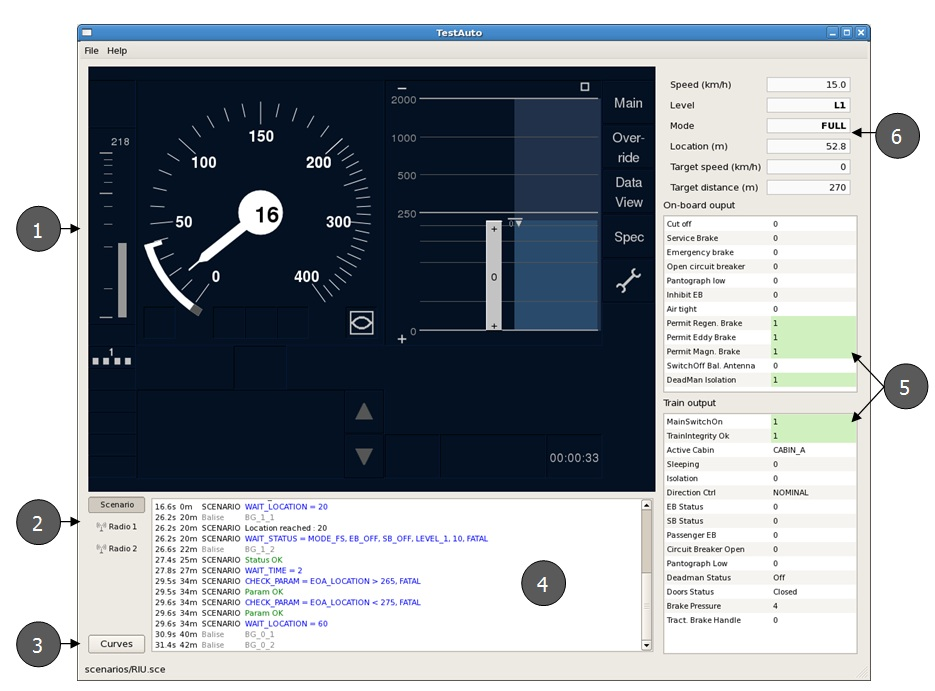
\includegraphics[width=\textwidth]{image/test_runner_GUI}
  \caption{Main window}
  \label{fig:Main window}
\end{figure}
Description : 
\begin{enumerate}
\item Integrated ERA DMI
\item Logs selector. Default is “Scenario”.
\item Curve window button
\item Logs display
\item TIU : Output of train and on-board
\item Odometric data and internal status
\end{enumerate}
\newpage
\subsubsection{DMI}
Driver actions of a scenario are simulated on the DMI by automated clicks. For each driver action the sequence of clicks are saved in a configuration file .testrunner\_rc located in the folder of the test runner application.
\newline
\newline 
Example:
\newline 
\fcolorbox{gray}{gray}{\begin{minipage}{\textwidth}
	DriverID = "click(600,350);wait(200);click(500,110);wait(850);"
\end{minipage}}
\newline
\newline  
The command wait(time) permit the software to update content (display, data) before the next click. All commands shall be separated by a semicolon.
Display of automated clicks is represented by a red circle on the DMI.
\newline 
\begin{figure}[!h]
  \centering
  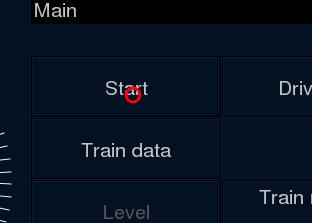
\includegraphics{image/test_runner_auto_click}
  \caption{An automated click on Start}
  \label{fig:An automated click on Start}
\end{figure}
\newline 
\emph{Warning :} User actions on DMI are not inhibited. Therefore, it is not recommended to interact with the DMI during a test execution.
\newpage
\subsubsection{Logs view}
The logs views informs user about:
\begin{itemize}
\item Executed commands
\item Results of tests
\item Trackside messages
\item On-board messages
\end{itemize}
Messages can be displayed in a separated window by double-clicking on them.
\newline
\newline
\begin{figure}[!h]
  \centering
  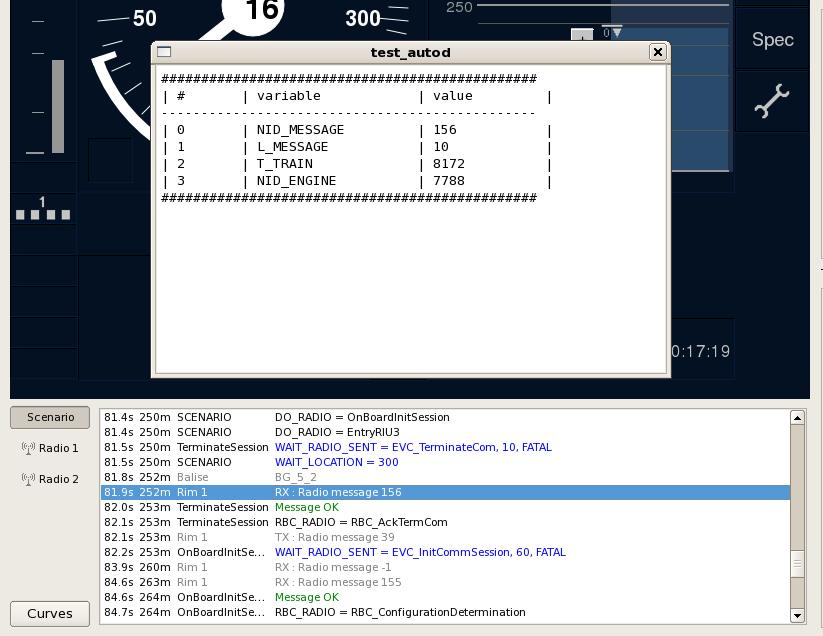
\includegraphics[width=\textwidth]{image/test_runner_message_window}
  \caption{Message window}
  \label{fig:Message window}
\end{figure}
\newline
\newline
\emph{Radio 1} and \emph{Radio 2} logs give status of the connection with the on-board. A green icon is displayed when connection is established with on-board.
At the end of the scenario execution, the result is displayed:
\begin{itemize}
\item SUCCESS: the scenario has been executed until end successfully
\item FAILURE: the scenario execution has been interrupted during execution due to an error in the scenario or a ‘FATAL’ argument in a condition test that has not been fulfilled.
\end{itemize}
\newpage
\subsubsection{Curve supervision display}
Curve window display supervision curve computed by on-board. This window can be switched on/off by clicking Curve button on the main window.
\begin{figure}[!h]
  \centering
  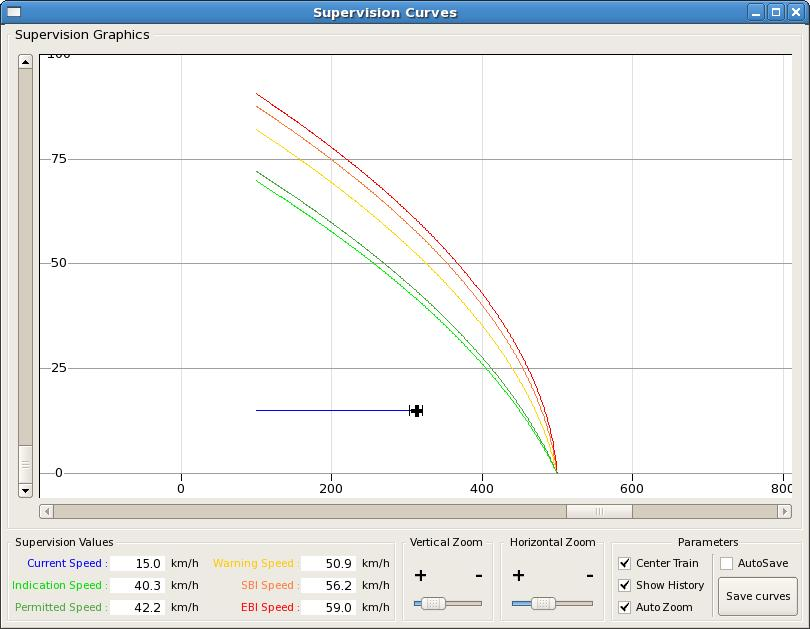
\includegraphics[width=\textwidth]{image/test_runner_supervision_curves}
  \caption{Curve window}
  \label{fig:Curve window}
\end{figure}
Options on the bottom right of the window allow user to adjust the view. 
A save function is available to record all points in a single CSV file in the data/curve/ directory.
%\subsection{Multiple scenario execution}
%It is possible to run the whole set of scenarios contained in the scenario/ directory by calling the provided script:
%\newline
%\newline
%\fcolorbox{gray}{gray}{\begin{minipage}{\textwidth}
%	>./runAllScenarios.py
%\end{minipage}}
%\newline
%\newline
%During the execution, the script generates an execution summary and backups some log files.
%The log file archive contains:
%\begin{itemize}
%\item On-board log files from the data/log/ directory
%\item The generated JRU file
%\end{itemize}
%The execution summary (<date>-<time>-allresults.txt) contains for each scenario the execution result:
%\begin{itemize}
%\item SUCCESS: the scenario has been executed until end successfully.
%\item EXPECTED FAILLURE: the scenario has failed but this is attended since the bug is not yet implemented (because the scenario was configured with %“EXPECTED\_TO\_FAIL”) or the scenario requires some special configuration to be executed (ex: “DMI\_SIMPLIFIED\_SUPPORTED” command).
%\item REGRESSION FAILURE: the scenario execution has been interrupted during execution due to an error in the scenario or a ‘FATAL’ argument in a condition test %that has not been fulfilled.
%\item SYNTAX: the scenario has failed because one command was not recognized or not used correctly.
%\item JITTER: sometimes, errors happen because of random issues. To detect this, in case of a failure, we launch the test 3 times. If it doesn’t fail every time, %we mark the result with this tag.
%\item UNKNOWN-ERROR: the scenario execution has terminated but result is unknown.
%\end{itemize}
%\fbox{\begin{minipage}{\textwidth}
%	\begin{description}
%		\item[] 1/14: Scenario 'Adhesion' ... SUCCESS
%		\item[] 2/14: Scenario 'AxleLoadOK' ... SUCCESS
%		\item[] 3/14: Scenario 'AxleLoadSB' ... SUCCESS
%		\item[] 4/14: Scenario 'BGError' ... SUCCESS
%		\item[] 5/14: Scenario 'Backward\_mvt' ... SUCCESS
%		\item[] 6/14: Scenario 'BadBGVersion' ... FAILURE
%		\item[] 7/14: Scenario 'Bad\_RBC\_version' ... SUCCESS
%		\item[] 9/14: Scenario 'CheckEOA' ... SUCCESS
%		\item[] 10/14: Scenario 'ConditionalLevelTransition\_0\_1' ... SUCCESS
%		\item[] 11/14: Scenario 'ConditionalLevelTransition\_0\_2' ... SUCCESS
%		\item[] 12/14: Scenario 'UnlkBGMissedBG' ... SUCCESS
%		\item[] 14/14: Scenario 'UnlkInvBG2’ ... FAILURE
%	\end{description}
%	TOTAL=21 – UNKNOWN-ERROR=0 - FAILURE=2 - SUCCESS=12
%\end{minipage}}
\newpage
\section{Example of scenario file}
\begin{lstlisting}[frame=single]
# test scenario definition
# start in level 1, move and transition to level 2


[SCENARIO]

# SoM in level 1

DRIVER_ACTION	= MainSwitchOn
WAIT_STATUS		= MODE_SB, 2, FATAL
DRIVER_ACTION	= OpenCabinA, 2
DRIVER_ACTION	= DriverID, 2
WAIT_TIME		= 1
DRIVER_ACTION	= Level1
WAIT_TIME		= 1
DRIVER_ACTION	= TrainData
WAIT_TIME		= 1
DRIVER_ACTION	= StartOfMission
WAIT_TIME		= 1
DRIVER_ACTION	= ACK

WAIT_STATUS	= LEVEL_1, EB_OFF, SB_OFF, MODE_SR, 5, FATAL

DRIVER_ACTION = DirectionNominal
MOVE_TRAIN

WAIT_LOCATION = 30

DO_RADIO = Connection+MA


# wait TAF to level border
WAIT_LOCATION = 100
WAIT_RADIO_SENT = MArequestFree, 5, FATAL


# wait level transition location
WAIT_LOCATION = 130

WAIT_STATUS = LEVEL_2, EB_OFF, SB_OFF, MODE_FS, 5, FATAL

WAIT_LOCATION = 530
WAIT_STATUS = LEVEL_2, EB_OFF, SB_OFF, MODE_FS, 5, FATAL


# ---------------------- Radio Procedures ---------------------

[Connection+MA]
WAIT_RADIO_SENT = InitCommSession, 10, FATAL
RBC_RADIO		= ConfigurationDetermination
WAIT_RADIO_SENT = SessionEstablished, 5, FATAL
WAIT_RADIO_SENT = ValidatedTrainData, 5, FATAL
RBC_RADIO		= AckTrainData
RBC_RADIO		= MA



# --------------------- RBC telegrams -------------------------

[ConfigurationDetermination]
NID_MESSAGE = 32
NID_LRBG	= 1
M_VERSION = 16d

[AckTrainData]
NID_MESSAGE = 8
NID_LRBG	= 1

[MA]
NID_MESSAGE = 3
NID_LRBG	= 1
# MA data 
NID_PACKET	= 15
Q_DIR		= 1
Q_SCALE		= 1
L_ENDSECTION = 5000
# SSP
NID_PACKET	= 27
Q_DIR		= 1
Q_SCALE		= 1
V_STATIC	= 60
# Gradient
NID_PACKET	= 21

# ------------------------ EVC telegrams ----------------------

[InitCommSession]
NID_MESSAGE = 155

[SessionEstablished]
NID_MESSAGE = 159

[ValidatedTrainData]
NID_MESSAGE = 129
NID_PACKET = 0
NID_PACKET = 11


[MArequestFree]
NID_MESSAGE = 132
NID_PACKET = 9
NID_LTRBG  = 11


# -------------------------- Balises --------------------------

[BaliseTrackside]
# announcement of level transition
30 = BG1_1
35 = BG1_2

# TAF free to L2 border
100 = BG2_1
105 = BG2_2

[BG1_1]
N_PIG	= 0
N_TOTAL = 1
NID_C	= 0
NID_BG	= 1
Q_LINK	= 1
# level transition packet
NID_PACKET		= 41
Q_DIR			= 1
Q_SCALE			= 1
D_LEVELTR		= 100
M_LEVELTR		= 3
L_ACKLEVELTR	= 50
# order to contact RBC
NID_PACKET		= 42
Q_DIR			= 1
Q_RBC			= 1
# Ending packet
NID_PACKET = 255

[BG1_2]
N_PIG	= 1
N_TOTAL = 1
NID_C	= 0
NID_BG	= 1
Q_LINK	= 1
# Ending packet
NID_PACKET = 255


[BG2_1]
N_PIG	= 0
N_TOTAL = 1
NID_C	= 0
NID_BG	= 2
Q_LINK	= 1
# TAF free to level 2 border
NID_PACKET		= 90
Q_DIR			= 1
NID_BG			= 11
# Ending packet
NID_PACKET = 255

[BG2_2]
N_PIG	= 1
N_TOTAL = 1
NID_C	= 0
NID_BG	= 2
Q_LINK	= 1
# Ending packet
NID_PACKET = 255




# ------------------------ Speed Profile ----------------------

[SpeedProfile]
0 = 0
500 = 40
1000 = 0

# ------------------------ configuration ----------------------


[Config_EVCInit]
LINE_LEVEL	= 1
COUNTRY_ID	= 0
GROUP_ID	= 4522
DISTANCE	= 50
DIRECTION	= NOMINAL
VALIDITY	= VALID

[Config_TrainData]
ETCS_ID		= 4554
BALISEANTENNA_OFFSET = 10
TRAIN_CATEGORY = 1
LOADING_GAUGE_MASK = 1
AXLE_LOAD = 237000
TRACTION_POWERS = 0, 1, 5, 41, 78, 11
TRAIN_LENGTH = 100
TRAIN_MASS = 142000.0
TRAIN_MAXACCEL = 0.5
SPEED_MAX = 300
EB_TIME = 1.0
EB_TIME = 1.0
CUTOFF_TIME = 1.0
BALISE_COM_AVAILABLE		= 1
LOOP_COM_AVAILABLE		= 1
RADIO_COM_AVAILABLE		= 1
INTEGRITY_DEVICE_AVAILABLE	= 1
SERVICE_BRAKE_AVAILABLE		= 1
ETCS_PHONE1                     = 1234123412341234
ETCS_PHONE2                     = 1234123412341235


[Config_SRSNationalDefaults]
COUNTRY_ID = 0
DRIVER_ADHESION = 0 
SH_SPEED = 30
SR_SPEED = 40
OS_SPEED = 30
UN_SPEED = 100
RELEASE_SPEED = 40
ROLLAWAY_DISTANCE = 2
SB_USETOTARGET = 1
EB_RUNRELEASE = 0
OVERRIDEEOA_ENTRYSPEED = 0
OVERRIDEEOA_MAXSPEED = 30
OVERRIDEEOA_MAXDISTANCE = 200
OVERRIDEEOA_MAXTIME = 60
DRIVERID_RUNCHANGE = 1

 
\end{lstlisting}
%===================================================
%Do NOT change anything below this line

\end{document}


\end{document}